%\documentclass[handout]{beamer}
\documentclass{beamer}
\usepackage{algorithm2e}
\usepackage{natbib}
\usepackage{layouts}
%\usepackage{enumitem}
%\usepackage[dvipsnames]{xcolor}
\definecolor{vuborange}{rgb}{1.0,0.40,0.0}
\definecolor{forestgreen}{rgb}{0.13, 0.55, 0.13}
\usetheme{Boadilla}
\usepackage{color,soul}
\usepackage{xcolor}
\usepackage{adjustbox}
\usepackage{amsmath,amssymb}
\usepackage{tikzsymbols}
\usepackage{booktabs}
\usepackage{calc}
\usepackage{subcaption}
\usepackage{graphicx}
\usepackage{tikz}
\usepackage{tikz-qtree}

%\newcommand\citet[1]{\citeauthor{#1}~\citeyear{#1}}
\usepackage[bordercolor=white,backgroundcolor=gray!30,linecolor=black,colorinlistoftodos]{todonotes}
\newcommand{\rework}[1]{%
	\todo[color=yellow,inline]{Rework: {#1}}%
}

\usetikzlibrary{shapes.geometric, arrows}

\title{Efficiently Explaining CSPs with Unsatisfiable Subset Optimization}
\institute[shortinst]
{\inst{1} Vrije Universiteit Brussel, Belgium \\ % Your institution for the title page
	\inst{2} KULeuven, Belgium \\ % Your institution for the title page
	\href{mailto:emilio.gamba@vub.be}{\underline{emilio.gamba@vub.be}}, \href{mailto:bart.bogaerts@vub.be}{bart.bogaerts@vub.be}, \href{mailto:tias.guns@kuleuven.be}{tias.guns@kuleuven.be} % Your email address
}
\date{ModRef 2022}
\author{\underline{Emilio Gamba}\inst{1} \and  Bart Bogaerts\inst{1} \and   Tias Guns\inst{1,2}}

\newcommand\hlyellow[1]{\hl{ {\sethlcolor{yellow}#1}}}
\newcommand\hlgreen[1]{\sethlcolor{green}\hl{#1}}

\tikzstyle{startstop} = [rectangle, rounded corners, minimum width=2cm, minimum height=0.5cm,text centered, draw=black]
\tikzstyle{io} = [trapezium, trapezium left angle=70, trapezium right angle=110, minimum width=3cm, minimum height=1cm, text centered, draw=black, fill=blue!30]
\tikzstyle{process} = [rectangle, minimum width=3cm, minimum height=1cm, text centered, draw=black, fill=orange!30]
\tikzstyle{decision} = [diamond, minimum width=3cm, minimum height=1cm, text centered, draw=black, fill=green!30]
\tikzstyle{arrow} = [thick,->,>=stealth]


\newcommand\m[1]{\ensuremath{\mathcal{#1}}\xspace}
\newcommand\allconstraints{\m{T_P}}
\newcommand\theory{\ensuremath{\m{F} }\xspace}
\newcommand\formula{\ensuremath{\m{F} }\xspace}
\newcommand\formulac{\ensuremath{\m{C} }\xspace}
\renewcommand\emph[1]{{\color{vuborange}#1}}
\newcommand\Iend{\m{I_{\mathit{end}}}}
\newcommand\Ipartial{\m{I}}
\newcommand\factexpl{fact\xspace}
\newcommand\LitsToExplain{DigitToExplain}

\newcommand\nat{\m{\mathbb{N}}}
\newcommand\subsetT{\m{\mathcal{S}}}
\newcommand\ltrue{\m{\textbf{t}}}
\newcommand\lfalse{\m{\textbf{f}}}
\newcommand\call[1]{\m{\textsc{#1}}}
\newcommand\onestep{\call{OneStep}}

\newcommand\muses[1]{\textsc{mus}s(\m{#1})}
\newcommand\mcses[1]{\textsc{mcs}s(\m{#1})}
%\begin{frame}{How to find OCUSs?}
%
%	
%\end{frame}

\newcommand\setstohit{\m{\mathcal{H}}}
\newcommand\grow{\call{Grow}}
\newcommand\sat{\call{SAT}}
\newcommand\corrss{\call{Correction-Subsets}}
\newcommand\comus{\call{ocus}}
\newcommand\cohs{\call{CondOptHittingSet}}
% \renewcommand{\labelitemi}{$\triangleright$}
\renewcommand{\thealgocf}{}


\makeatletter
\renewcommand{\@algocf@capt@plain}{above}% formerly {bottom}
\setbeamertemplate{footline}
{
	\leavevmode%
	\hbox{%
		\begin{beamercolorbox}[wd=.2\paperwidth,ht=2.25ex,dp=1ex,center]{author in head/foot}%
			\usebeamerfont{author in head/foot}Emilio Gamba (VUB)
		\end{beamercolorbox}%
		\begin{beamercolorbox}[wd=.6\paperwidth,ht=2.25ex,dp=1ex,center]{title in head/foot}%
			\usebeamerfont{title in head/foot}Efficiently Explaining CSPs with Unsatisfiable Subset Optimization
		\end{beamercolorbox}%
		\begin{beamercolorbox}[wd=.2\paperwidth,ht=2.25ex,dp=1ex,right]{date in head/foot}%
			\usebeamerfont{date in head/foot}ModRef 2022\hspace*{1em}
			\insertframenumber{} / \inserttotalframenumber\hspace*{2ex} 
	\end{beamercolorbox}}%
	\vskip0pt%
}
\makeatother

\begin{document}
	
	\begin{frame}
		\maketitle
		\begin{minipage}{0.45\textwidth}
			\begin{flushleft}
				
\includegraphics[width=\textwidth]{template_vub/VUB-AI_RGB-1-800x223}
			\end{flushleft}
		\end{minipage}		\hfill
	\begin{minipage}{0.15\textwidth}
	
	
\includegraphics[width=\textwidth]{figures/DTAI_Logo_2}
\end{minipage}
\hfill
	\begin{minipage}{0.15\textwidth}
		
		
\includegraphics[width=0.7\textwidth]{figures/datalab_400x400.jpg}
	\end{minipage}
	\end{frame}
	
	
%	\AtBeginSection[]
%	{
%		\begin{frame}
%			\frametitle{Outline}
%			\tableofcontents[currentsection]
%		\end{frame}
%	}
%	
%	\AtBeginSubsection[]
%	{
%		\begin{frame}
%			\frametitle{Outline}
%			\tableofcontents[currentsection,currentsubsection]
%		\end{frame}
%	}
%	

		\begin{frame}
\tableofcontents
	
\end{frame}			
	\begin{frame}
		
		\setlength{\textfloatsep}{0pt}
		\frametitle{Examples of Constraint Satisfaction Problems}
		\begin{minipage}[t]{0.45\textwidth}
			\begin{figure}[h]
				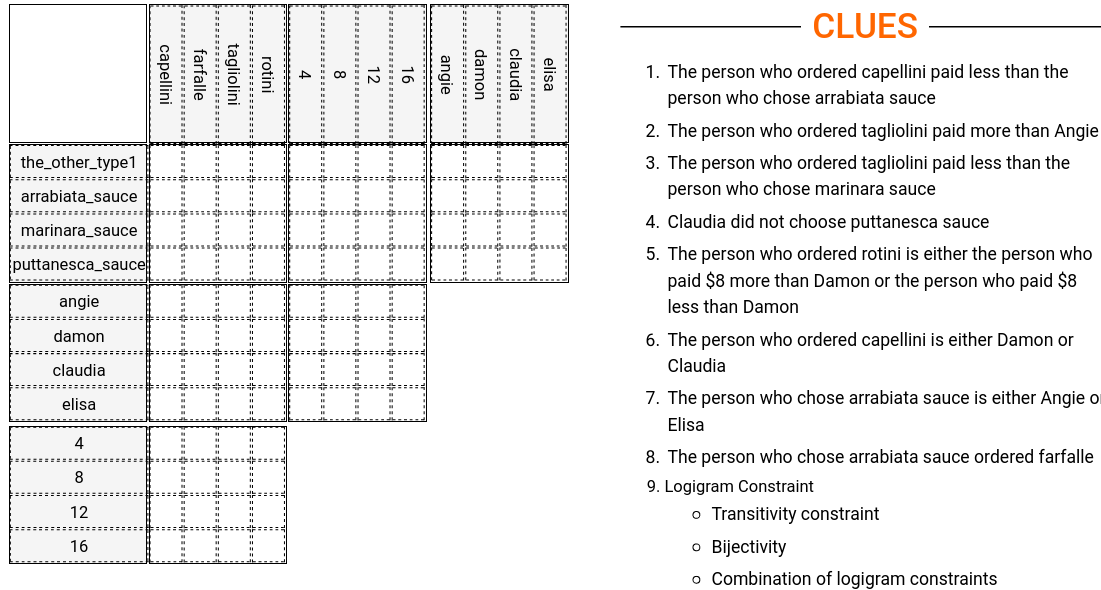
\includegraphics[width=\textwidth]{figures/logic_puzzle.png}
				\caption{\small Logic Grid Puzzle}
			\end{figure}
				\vspace{-8mm}
			\begin{figure}[h]
				\centering
				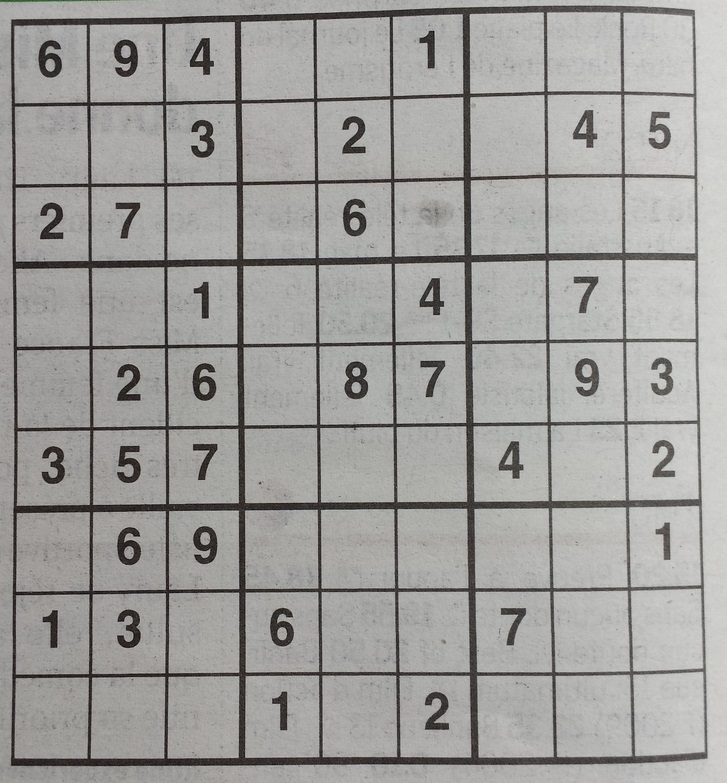
\includegraphics[width=.6\textwidth]{figures/sudoku_steps/sudoku.jpg}
				\caption{\small Sudoku}
			\end{figure}
		\end{minipage}
		\hfill
		\begin{minipage}[t]{0.52\textwidth}
			\begin{figure}[h]
				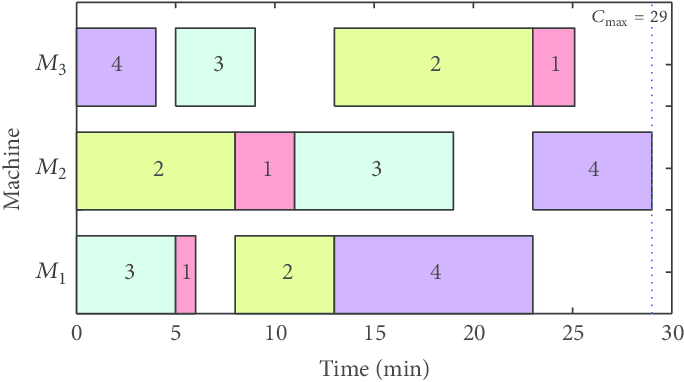
\includegraphics[width=\textwidth]{figures/scheduling.png}
				\caption{\small (Room) Scheduling Problem}
			\end{figure}
				\vspace{-8mm}
			\begin{figure}[h]
				\includegraphics[width=\textwidth]{figures/omus-presentation-car.png}
				\caption{\small (Car) configuration problems}
			\end{figure}
		\end{minipage}

	\end{frame}
	
	\section{Motivation}
\begin{frame}
	\frametitle{Constraint Satisfaction Problems}
	\framesubtitle{Solving}
	
	\begin{center}
		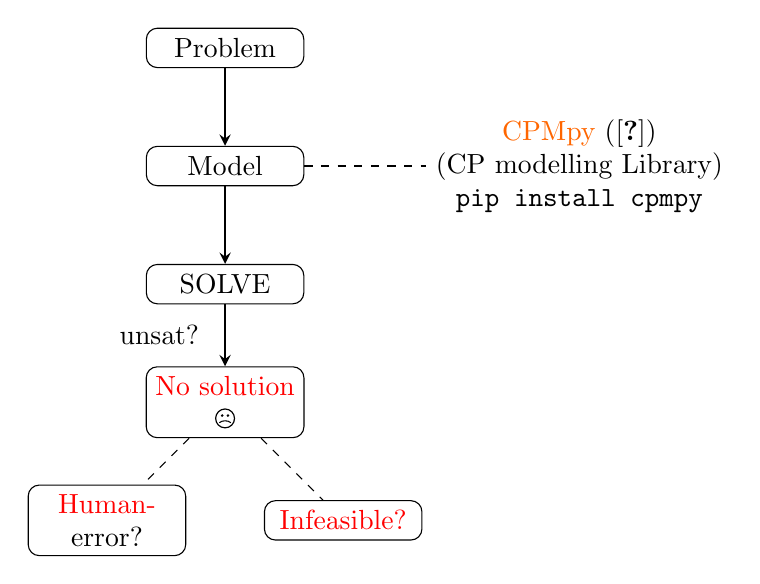
\begin{tikzpicture}[node distance=1.5cm]
			\node (problem) [startstop] {Problem};
			\pause
			\node (model) [startstop, below of=problem] {Model}; 
			\draw [arrow] (problem) -- (model);			
%			\node (Essence) [right of=model, xshift=1cm] {CPMpy \cite{CPMpy}}; 
			\node (cpmpy) [align=center, right of=model, xshift=3cm] {\emph{CPMpy} (\cite{guns2019increasing}) \\ (CP modelling Library) \\\texttt{pip install cpmpy}}; 
%			\node (Essence) [right of=model, xshift=1cm] {CPMpy \cite{CPMpy}}; 
			\draw [dashed] (model) -- (cpmpy);									
			\pause
			
			\node (solve) [startstop, below of=model] {SOLVE};
			\draw [arrow] (model) -- (solve); \pause
			
			\node  (modelerror) [startstop, below of=solve, align=center] {\color{red} No solution\\ \Sadey}; %todo: add smiley face sad
			\draw [arrow] (solve) --node[anchor=east,xshift=-0.2cm] {unsat?} (modelerror); 			
			\pause
			\node  (human) [startstop, below of=modelerror, xshift=-1.5cm, align=center] {\color{red} Human-\\error?}; %todo: doodle human
			\draw [dashed] (modelerror) --  (human); 
			\pause
			\node  (Infeasible) [startstop, below of=modelerror, xshift=1.5cm, align=center] {\color{red} Infeasible?}; 
			\draw [dashed] (modelerror) --  (Infeasible); 

		\end{tikzpicture}
	\end{center}
\end{frame}

\begin{frame}
	\frametitle{Constraint Satisfaction Problems}
	\framesubtitle{Solving}
			\begin{minipage}{0.4\textwidth}
		\begin{center}
			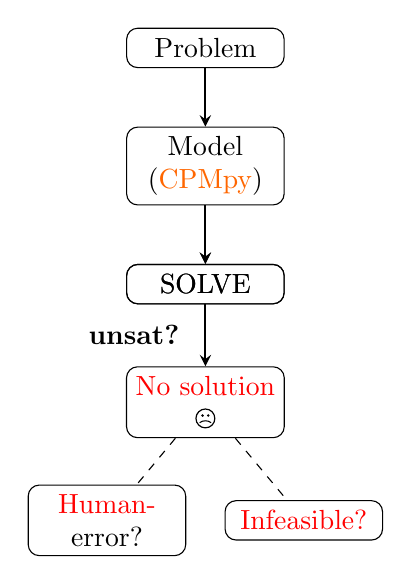
\begin{tikzpicture}[node distance=1.5cm]
				\node (problem) [startstop] {Problem}; 
				
				\node (model) [startstop, below of=problem,align=center] {Model \\ (\emph{CPMpy})}; 
				\draw [arrow] (problem) -- (model);			
				
%				\node (cpmpy) [right of=model, xshift=0.75cm] {CPMpy}; 
%				\draw [dashed] (model) -- (cpmpy);									
				
				\node (solve) [startstop, below of=model] {SOLVE};
				\draw [arrow] (model) -- (solve); 
			
			\node (solve) [startstop, below of=model] {SOLVE};
			\draw [arrow] (model) -- (solve); 

			\node  (modelerror) [startstop, below of=solve, align=center] {\color{red} No solution\\ \Sadey}; %todo: add smiley face sad
			\draw [arrow] (solve) --node[anchor=east,xshift=-0.2cm] {\textbf{unsat?}} (modelerror); 			
			\node  (human) [startstop, below of=modelerror, xshift=-1.25cm, align=center] {\color{red} Human-\\error?}; %todo: doodle human
			\draw [dashed] (modelerror) --  (human); 
			\node  (Infeasible) [startstop, below of=modelerror, xshift=1.25cm, align=center] {\color{red} Infeasible?}; 
			\draw [dashed] (modelerror) --  (Infeasible); 

				\end{tikzpicture}
		\end{center}
	\end{minipage}
	\begin{minipage}{0.59\textwidth}
	\textbf{How do you explain UNSAT ? } \\	
	\begin{figure}[H]
		\centering
	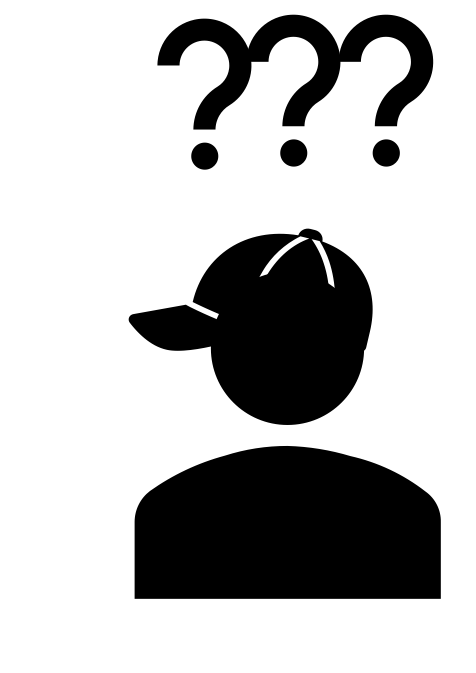
\includegraphics[width=0.3\textwidth]{figures/unsat/human.png}
	\end{figure}

%	\pause
%	\begin{itemize}
%		\item Extract a \emph{Minimum Unsatisfiable Subsets} (MUS) \pause
%		\item Enumerate all \emph{Minimum Unsatisfiable Subsets} (MUS) \pause
%		\item Extract a \emph{Minimum Correction Subsets} (MCS)
%		\begin{itemize}
%			\item \emph{Correct} your model by modifying a subset of the model constraints
%		\end{itemize}
%	\end{itemize}
	\end{minipage}
\end{frame}

\begin{frame}
	\frametitle{How do I debug my model}
	\framesubtitle{Explanations of unsatisfiability}
	

\begin{minipage}{0.7\textwidth}
	\only<1>{\hfill}
	 \only<2->{
\begin{enumerate}
	\item Identify conflicting constraints as an explanation  \footnotesize{(\cite{DBLP:journals/jar/LiffitonS08,ignatiev2015smallest}...)}
	\begin{itemize}
		\item[$\rightarrow$] Extract a \textbf{\textit{\color{red}Minimum Unsatisfiable Subset}} (\textbf{\textit{\color{red}MUS}}) 
		\item[=] Irreducible Inconsistent Subsystem (ISS) 
	\end{itemize}
 \only<3->{\item Identify a \textbf{\textit{\color{forestgreen}Maximal Satisfiable Subset}} (\textbf{\textit{\color{forestgreen}MSS}}) {\footnotesize{(\cite{ignatiev2019rc2,davies2013exploiting,hansen1990algorithms}...)}}} 
\only<4->{\item ``Correct'' the infeasibility in the constraints \footnotesize{(\cite{liffiton2013enumerating}...)}
	\begin{itemize}
	\item[$\rightarrow$] Extract a \textbf{\textit{\color{blue}Minimum Correction Subset}} (\textbf{\textit{\color{blue}MCS}})
	\item[=] Complement of some \textbf{\textit{\color{forestgreen}MSS}}, removal/correction leads to a satisfiable subset
\end{itemize}}
\end{enumerate}}

		\end{minipage}
	\begin{minipage}{0.28\textwidth}
	\only<1>{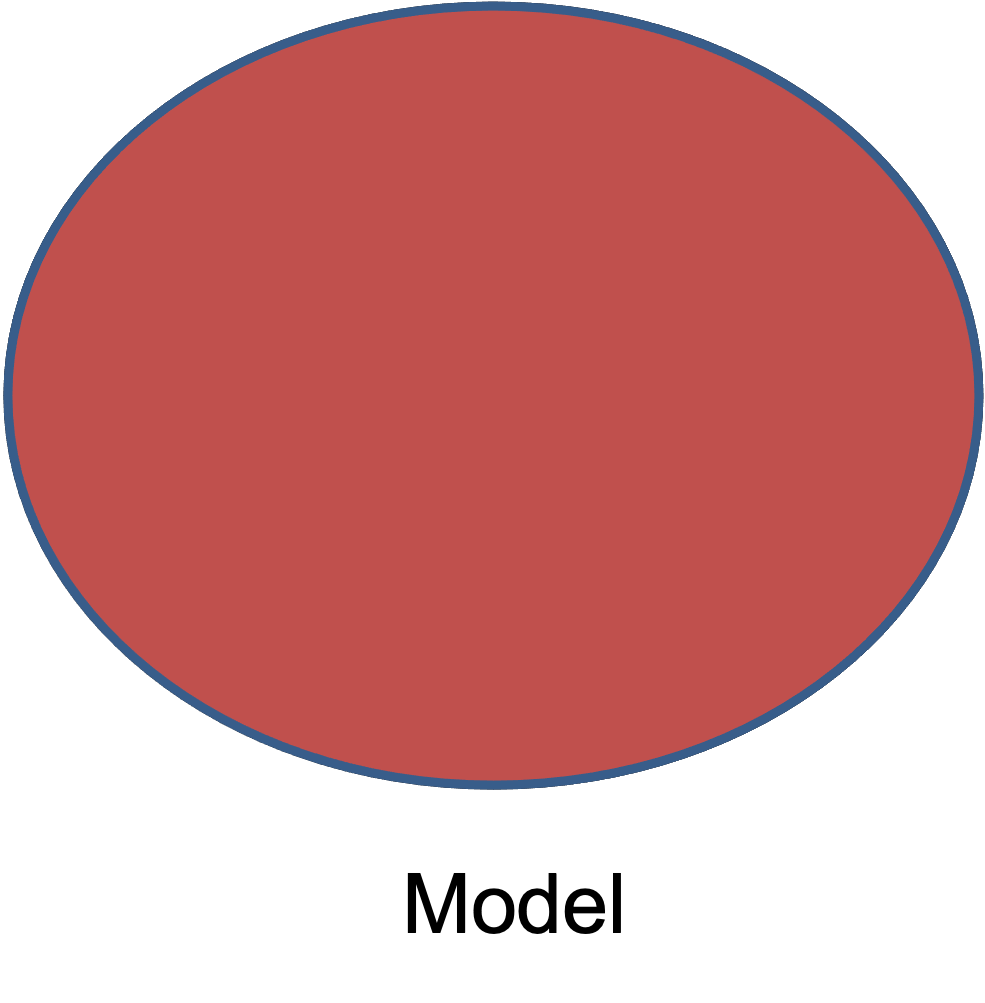
\includegraphics[width=\textwidth]{figures/unsat/model.png}}
	\only<2>{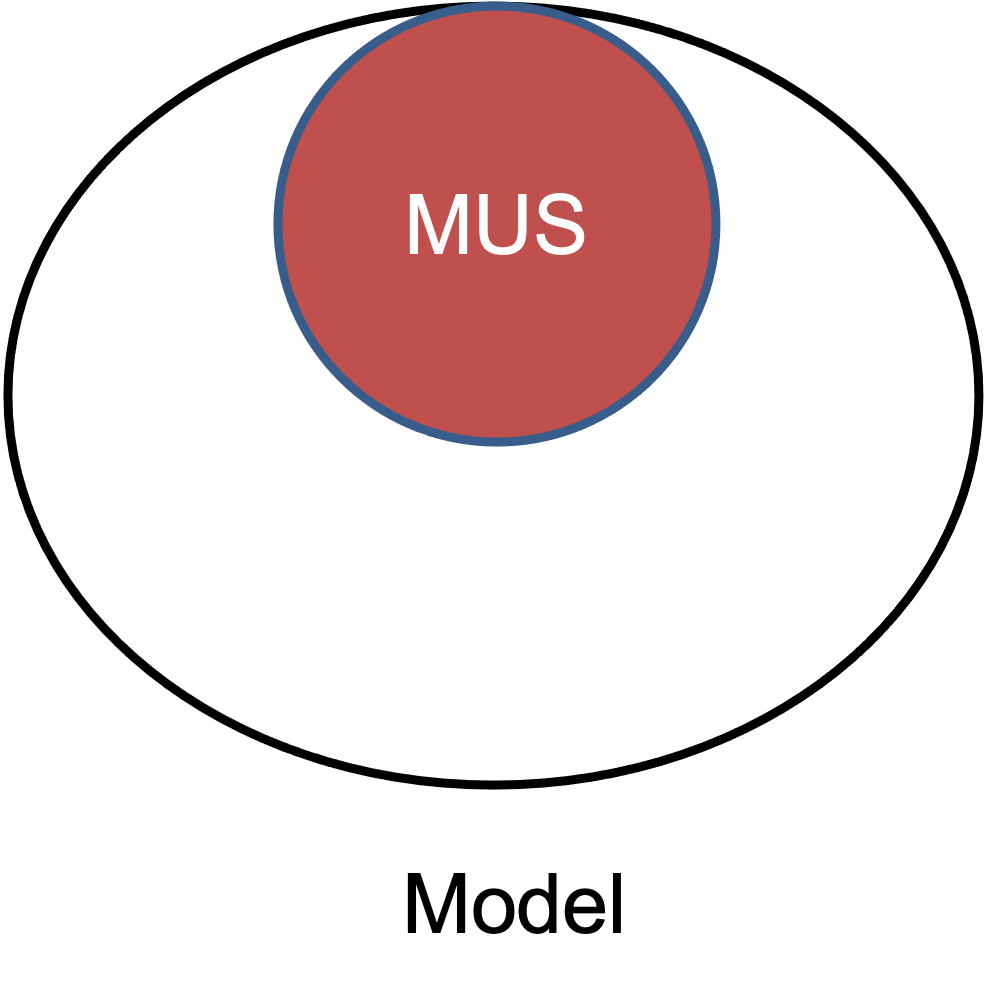
\includegraphics[width=\textwidth]{figures/unsat/mus.png}}
	\only<3>{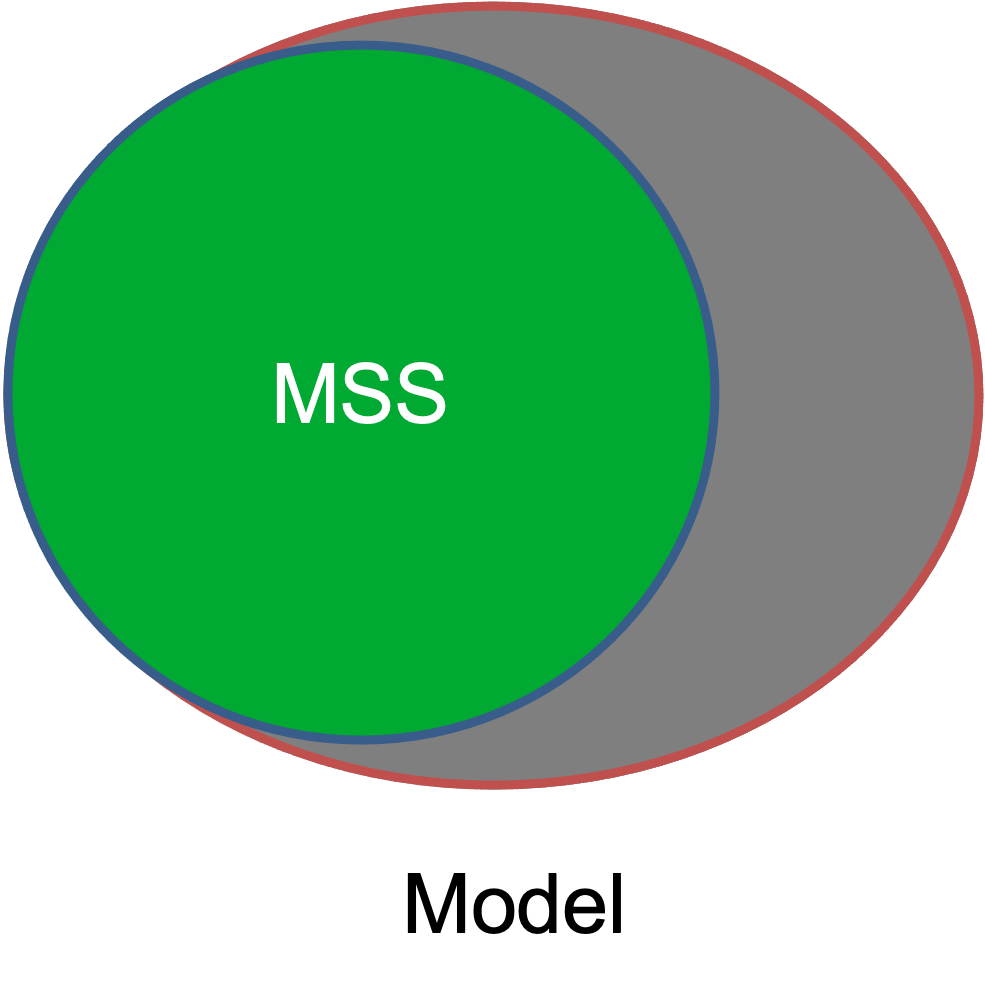
\includegraphics[width=\textwidth]{figures/unsat/mss.png}}
	\only<4>{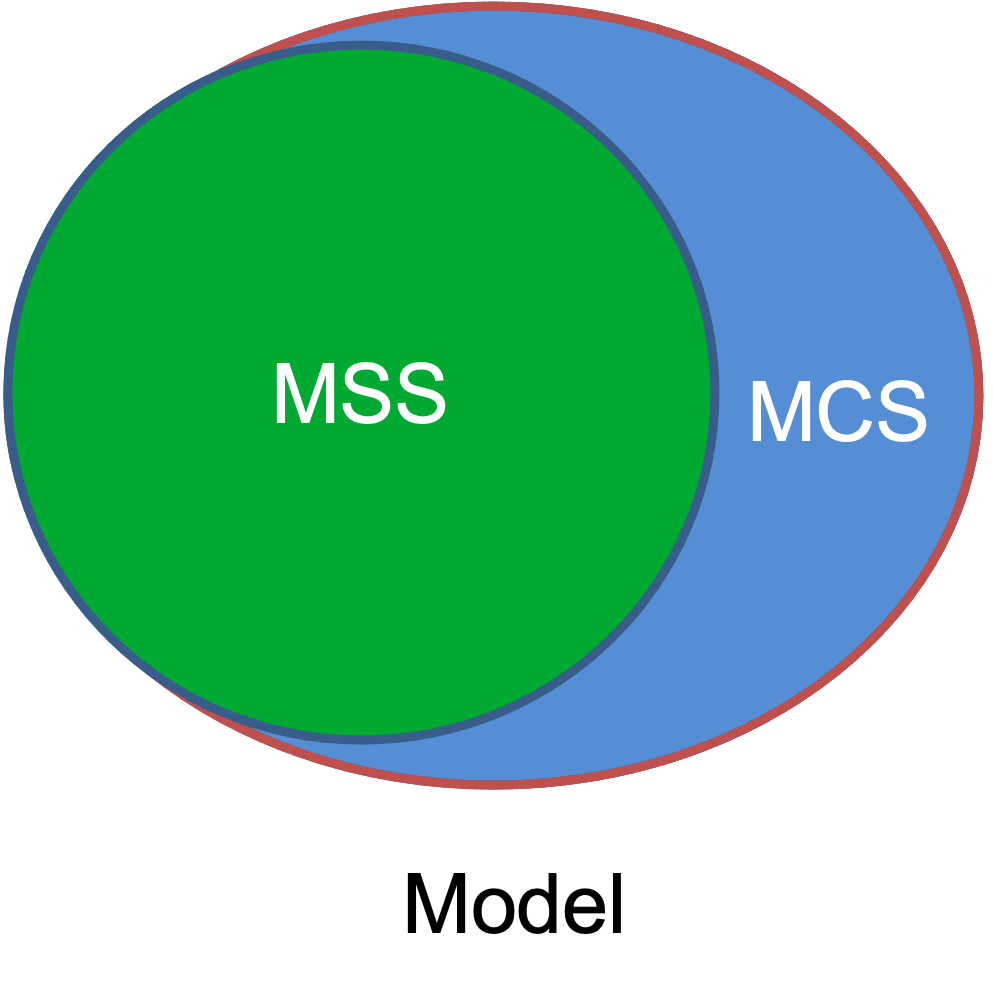
\includegraphics[width=\textwidth]{figures/unsat/msc.png}}
	\end{minipage}
\vfill
\end{frame}
	
	\section{How do I explain Satisfiability?}
	\begin{frame}
		\frametitle{Motivation - Explaining SAT problems}
		\begin{minipage}{0.35\textwidth}
			\begin{center}
				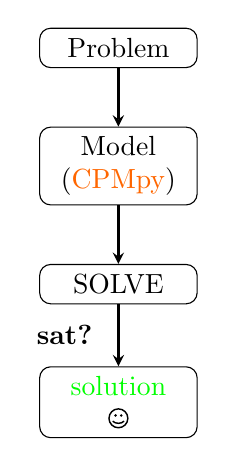
\begin{tikzpicture}[node distance=1.5cm]
					\node (problem) [startstop] {Problem}; 
					
				\node (model) [startstop, below of=problem,align=center] {Model \\ (\emph{CPMpy})}; 
				\draw [arrow] (problem) -- (model);								
					
					\node (solve) [startstop, below of=model] {SOLVE};
					\draw [arrow] (model) -- (solve); 
					
					%					\node  (modelerror) [startstop, below of=solve] {\color{red} modeling error?};
					%					\draw [arrow] (solve) --node[anchor=east,xshift=-0.2cm] {unsat?} (modelerror); 
					\node  (solution) [startstop, below of=solve,align=center]  {\color{green} solution\\ \Smiley};
					%						\node  (solution) [startstop, below of=sat] {\color{green} solution};
					%	
					\draw [arrow] (solve) --node[anchor=east,xshift=-0.2cm] {\textbf{sat?}} (solution);
					
					%						\draw [arrow] (sat) -- (solution);			
					
				\end{tikzpicture}
			\end{center}
		\end{minipage}
		\begin{minipage}{0.63\textwidth}
			\pause
			\textbf{How do I explain SAT ? }	\pause
			\begin{itemize}
				\item What is an \textbf{\emph{explanation}}? \pause
				\item What is a \emph{\textbf{good}} explanation ? \pause
				\item What is a \textbf{\emph{sequence of explanations}} ? 
			\end{itemize}
		\end{minipage}
		
	\end{frame}
	
	
%	\begin{frame}
%		\frametitle{Outline}
%		\tableofcontents
%	\end{frame}
%	

	\begin{frame}{What is an explanation ?}

			\only<1>{
				\begin{figure}[H]
					\centering
				\includegraphics[width=0.7\textwidth]{figures/sudoku_steps/sudoku-step1}
				\end{figure}
			}
					\only<2>{
				\begin{figure}[H]
	\centering
	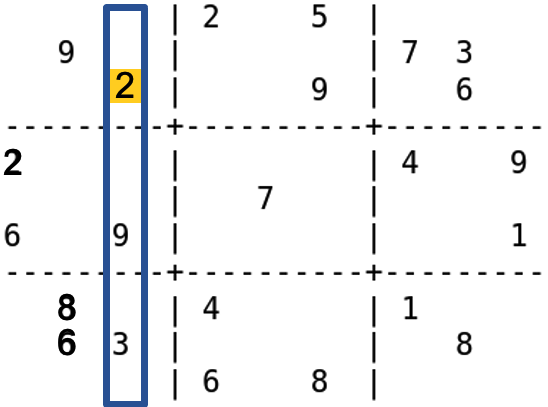
\includegraphics[width=0.7\textwidth]{figures/sudoku_steps/sudoku-step2}
\end{figure}
		}
				\only<3>{
				\begin{figure}[H]
	\centering
	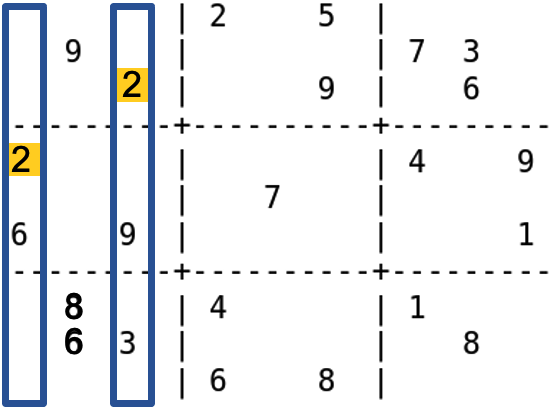
\includegraphics[width=0.7\textwidth]{figures/sudoku_steps/sudoku-step3}
\end{figure}
	}
			\only<4>{
				\begin{figure}[H]
	\centering
	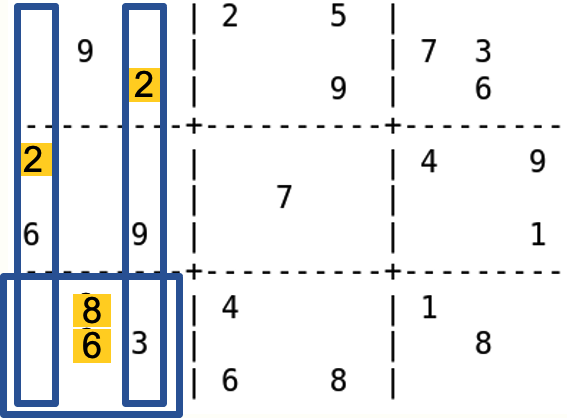
\includegraphics[width=0.7\textwidth]{figures/sudoku_steps/sudoku-step4}
\end{figure}
}
			\only<5>{
				\begin{figure}[H]
	\centering
	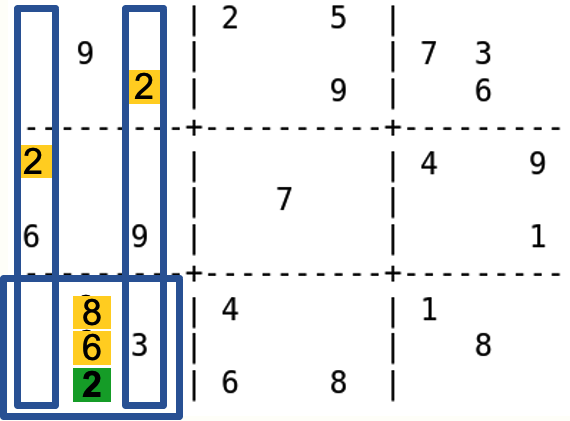
\includegraphics[width=0.7\textwidth]{figures/sudoku_steps/sudoku-step5}
\end{figure}
}
	\end{frame}

\begin{frame}
	\frametitle{Stepwise explanations for CSPs}
	\frametitle{What is a \emph{sequence} of explanations ?}
	
	\begin{minipage}{0.28\textwidth}
		\includegraphics[width=\textwidth]{figures/sudoku_sequence/sudoku-step1}
	\end{minipage}\hfill\pause
	\begin{minipage}{0.045\textwidth}
		\begin{center}
			$\rightarrow$
		\end{center}
	\end{minipage}\hfill
	\begin{minipage}{0.28\textwidth}
		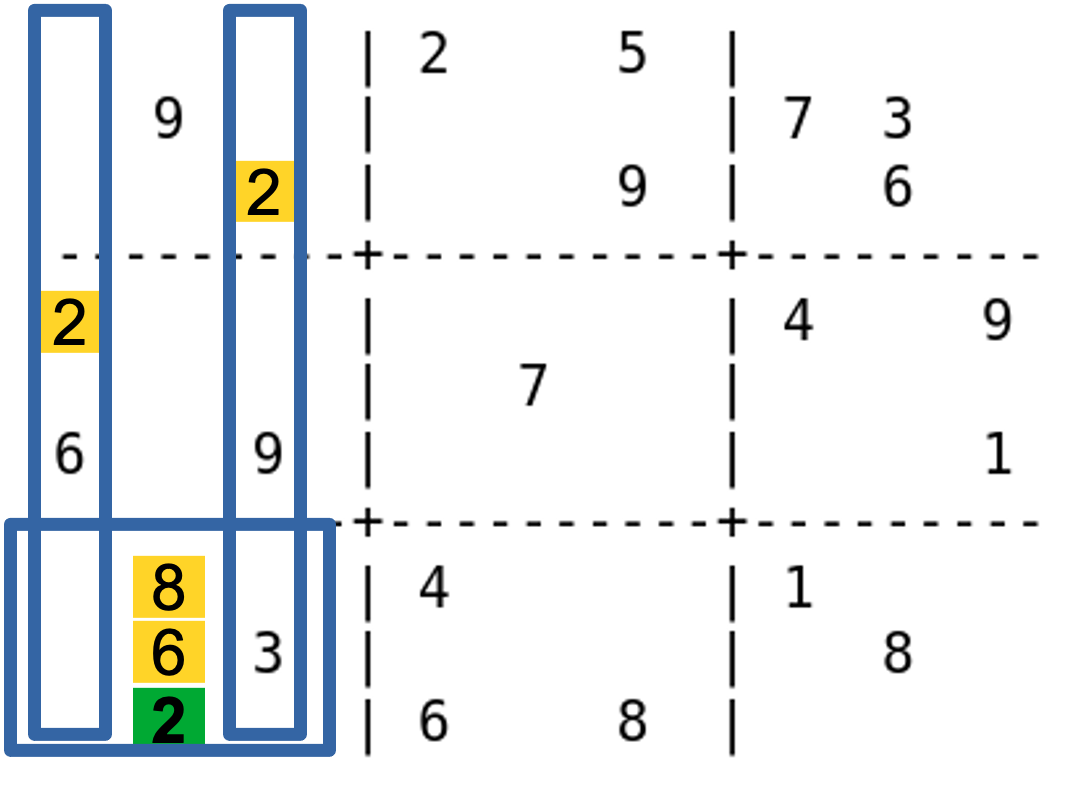
\includegraphics[width=\textwidth]{figures/sudoku_steps/sudoku3}
	\end{minipage}\hfill
	\begin{minipage}{0.045\textwidth}
		\begin{center}
			$\rightarrow$
		\end{center}
	\end{minipage}\hfill
	\begin{minipage}{0.28\textwidth}
		\begin{center}
			$\dots$
		\end{center}
	\end{minipage}\\\vfill \pause
	\begin{minipage}{0.28\textwidth}
		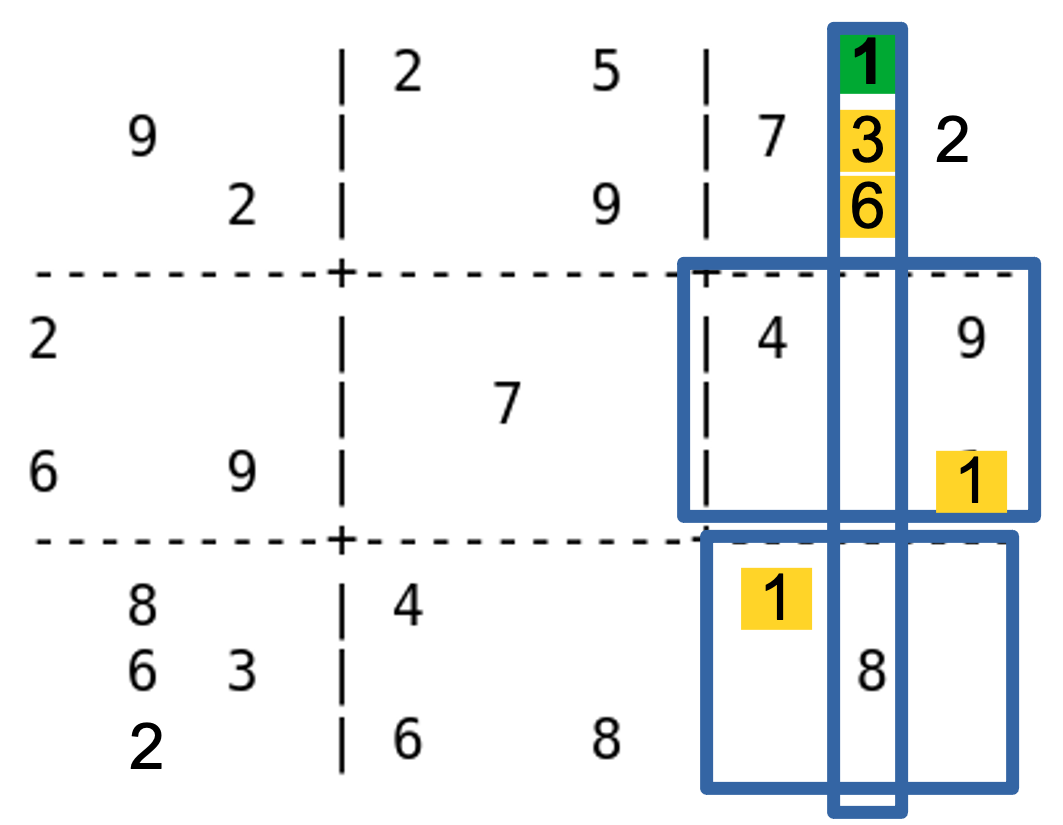
\includegraphics[width=\textwidth]{figures/sudoku_sequence/sudoku-step3}
	\end{minipage}
	\hfill
	\begin{minipage}{0.43\textwidth}
		\begin{center}
			$\rightarrow$ \hspace{0.5cm}\dots \hspace{0.5cm}$\rightarrow$
		\end{center}
	\end{minipage}\hfill\pause
	\begin{minipage}{0.28\textwidth}
		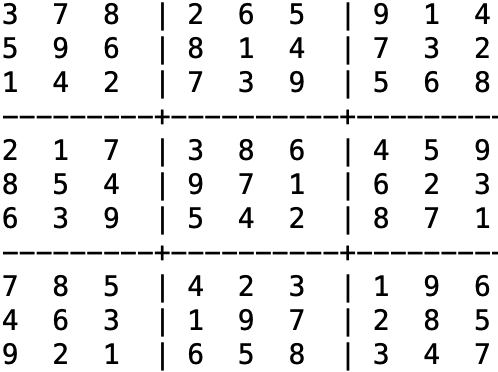
\includegraphics[width=\textwidth]{figures/sudoku_sequence/sudoku-stepn}
	\end{minipage}
\end{frame}

\begin{frame}
	\frametitle{Stepwise explanations for CSPs}
	\framesubtitle{Goal}

\textbf{Given}
\begin{itemize}
	\item[{
\includegraphics[width=15pt]{figures/explanation_steps/explanation_S_full}}] Constraints 
	\item[{
\includegraphics[width=15pt]{figures/explanation_steps/explanation_E_full}}] Facts, i.e. given sudoku numbers
\end{itemize} \pause
\vspace{20pt}
\textbf{Goal:}
\begin{itemize}
	\item[$\triangleright$] Generate a \textit{\emph{sequence}} of \textit{\emph{simple}} explanations \pause
	\item[$\triangleright$]  Explain step-by-step the solution of a Constraint Satisfaction Problem \pause 
	\item[$\triangleright$] Explain 1 fact at a time 
\end{itemize}

\end{frame}



	\begin{frame}{Stepwise explanations for CSPs}
		\framesubtitle{Explanation step - Formal definition}

      	Let an \emph{EXPLANATION STEP} (\citet{bogaerts2020step})  be:
      	\begin{center}
      		{\Large {
\includegraphics[width=15pt]{figures/explanation_steps/explanation_E}} $\&$ {
\includegraphics[width=15pt]{figures/explanation_steps/explanation_S}} $\implies$ {
\includegraphics[width=15pt]{figures/explanation_steps/explanation_N}}}
      	\end{center}
      	
      \begin{minipage}{0.65\textwidth}
      	\only<1>{\hfill}
      	\only<2->{
      	\begin{itemize}
      		\item[{
\includegraphics[width=15pt]{figures/explanation_steps/explanation_E}}] A subset of previously derived facts 
\includegraphics[width=10pt]{figures/explanation_steps/explanation_E_full} 
      		\begin{itemize}
				\item[\textit{(Sudoku)}] Given and derived digits in the grid 
      		\end{itemize}
      	\only<3->{
      		\item[{
\includegraphics[width=15pt]{figures/explanation_steps/explanation_S}}] A minimal subset of model constraints 
\includegraphics[width=10pt]{figures/explanation_steps/explanation_S_full}
      		\begin{itemize}
				\item[\textit{(Sudoku)}] Alldifferent column, row, box constraints 
			\end{itemize}}
		\only<4->{
      		\item[{
\includegraphics[width=15pt]{figures/explanation_steps/explanation_N}}] A newly derived fact s.t.       		{ {
\includegraphics[width=7pt]{figures/explanation_steps/explanation_E}} $\&$ {
\includegraphics[width=7pt]{figures/explanation_steps/explanation_S}} $\implies$ {
\includegraphics[width=7pt]{figures/explanation_steps/explanation_N}}}}
      	\end{itemize}}
      \hfill
      \end{minipage}
        \begin{minipage}{0.34\textwidth}
			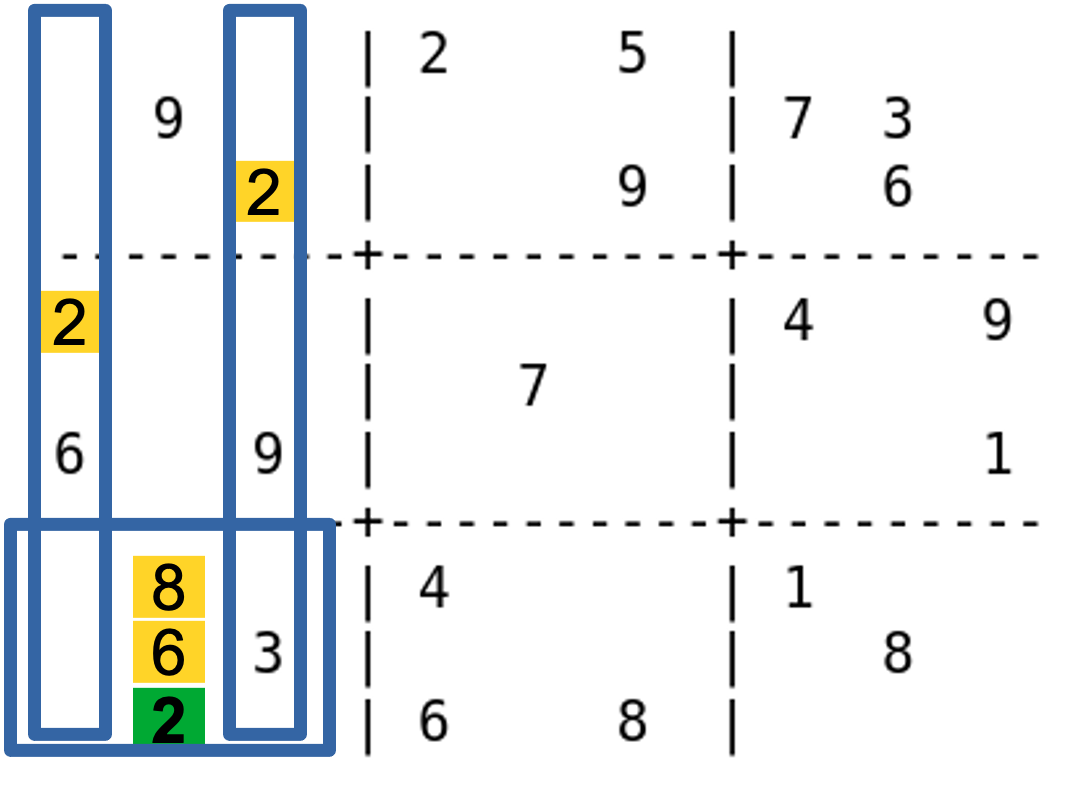
\includegraphics[width=\textwidth]{figures/sudoku_steps/sudoku3}
  \end{minipage}

      	\vfill
\only<5->{
\begin{center}
{\Large \textbf{How ?} \pause \large $\mathtt{\mathbf{MUS}}($ 
\includegraphics[width=10pt]{figures/explanation_steps/explanation_E_full} $\&$ {
\includegraphics[width=10pt]{figures/explanation_steps/explanation_S_full}} $\& \lnot$ {
\includegraphics[width=10pt]{figures/explanation_steps/explanation_N}} $)$ \textbf{is a valid explanation step}}
\end{center}
\vfill
}

	\end{frame}
	
	
%		\begin{frame}{Stepwise explanations for CSPs}
%		\framesubtitle{EXPLANATION STEP}
%		%		In, we introduce \emph{explanation} steps \pause
%		
%		\begin{example} (Sudoku) A traditional Constraint Satisfaction Problem (CSP) can be represented as a triple $CSP = ({\cal V},{\cal D},{\cal C})$ with variables ${\cal V}$, domain ${\cal D}$ and constraint set ${\cal C}$. Let $V_{(r, c)}$, ${\cal D}(V_{(r,c)}) = \{1,...,9\}$ be the decision variables of the 9x9 Sudoku CSP.\\ %. Let ${\cal C } $ be the alldiferent constraints such that: 
%			
%			
%			Let ${\cal C } $ be the alldiferent constraints such that: 
%			%				\begin{itemize}
%				%					\item all different digits on the same row $r$,  \\  
%				%					\item $\forall r \in 1 .. 9: \mathtt{alldifferent}(\{V_{(r,c)} | c \in 1 .. 9 \} )$; \\
%				$\forall r \in 1 .. 9: \mathtt{alldifferent}(\{V_{(r,c)} | c \in 1 .. 9 \} )$; \\
%				%					\item all different digits in the same column $c$  \\ 
%				%					\item $\forall c  \in 1 .. 9: \mathtt{alldifferent}(\{V_{(r,c)} | r \in {1 .. 9}\} )$ ; \\
%				$\forall c  \in 1 .. 9: \mathtt{alldifferent}(\{V_{(r,c)} | r \in {1 .. 9}\} )$ ; \\
%				%					\item all different digits in the same block   \\ 
%				%					\item $\forall b_r, b_c  \in 0 .. 2  : \mathtt{alldifferent}(\{ V_{(r_i ,c_j)} | $ \\ $r_i  \in 3b_r+ 1$ $..$ $3b_r+3 ,  c_j \in 3b_c + 1$ $..$  $3b_c + 3 \} )$.
%				$\forall b_r, b_c  \in 0 .. 2  : \mathtt{alldifferent}(\{ V_{(r_i ,c_j)} | r_i  \in 3b_r+ 1 .. 3b_r+3$,  $c_j \in 3b_c + 1$ $..$  $3b_c + 3 \} )$.
%				%				\end{itemize}
%		\end{example}
%	\end{frame}
	\begin{frame}{Stepwise explanations for CSPs}
		\framesubtitle{EXPLANATION STEP}
		%		In, we introduce \emph{explanation} steps \pause
		
		\begin{example} (Sudoku)
			Let $E$ contain the assigned variables at the current state of the grid (e.g. $I = \{V_{(3, 3)}  = 2, \dots \}$).
			
			\begin{minipage}{0.63\textwidth}
				{\Large $\mathtt{\mathbf{MUS}}($}{\large 
\includegraphics[width=10pt]{figures/explanation_steps/explanation_S_full} $\&$ {
\includegraphics[width=10pt]{figures/explanation_steps/explanation_E_full}} $\& \lnot$ {
\includegraphics[width=10pt]{figures/explanation_steps/explanation_N}} $)$ } \\ 
				
				$\{\mathtt{alldifferent}(\{V_{(r,1)} | r \in {1 .. 9}\}), V_{(4, 1)}  = 2$,\\
				$\mathtt{alldifferent}(\{V_{(r,3)} | r \in {1 .. 9}\}), V_{(3, 3)}  = 2$, \\  
				$\mathtt{alldifferent}(\{ V_{(r_i ,c_j)} | r_i  \in 7..9 ,  c_j \in 1..3 \})$,\\  
				$V_{(7, 2)}  = 2,V_{(8, 2)}  = 2, 	 V_{(9, 2)}  \neq 2\} $
			\end{minipage}
			\begin{minipage}{0.36\textwidth}
				\begin{figure}[H]
					\centering
					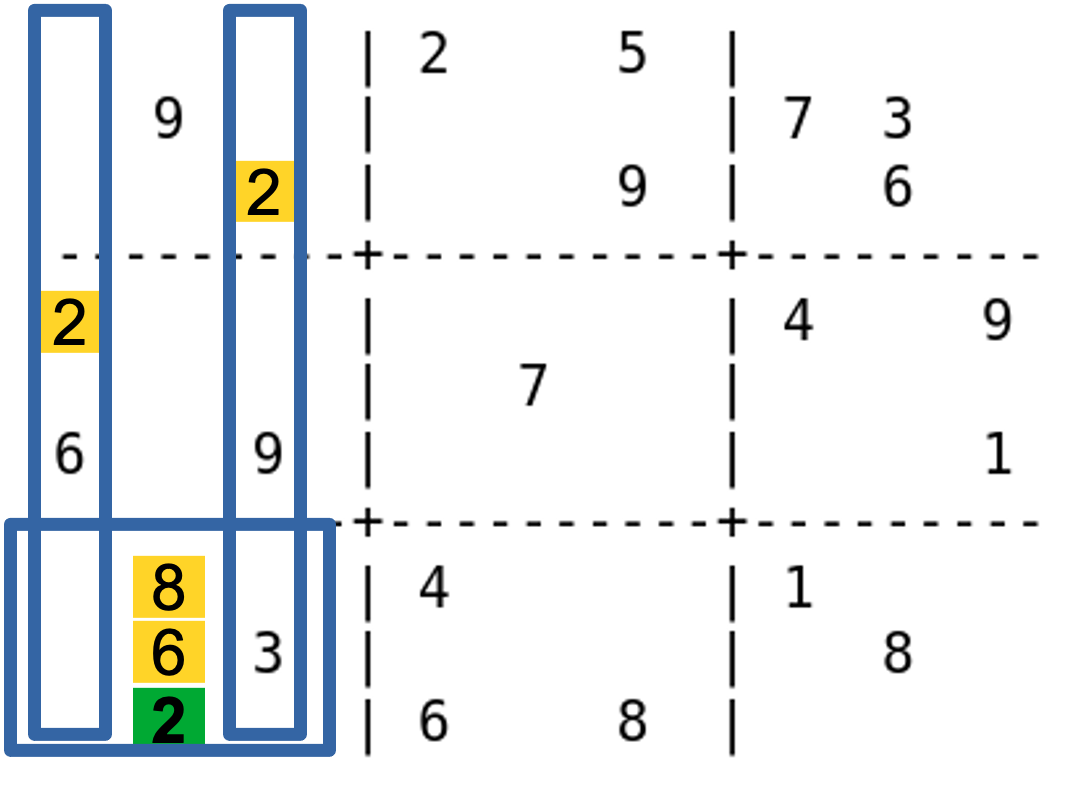
\includegraphics[width=\textwidth]{figures/sudoku_steps/sudoku3}
					\caption{Example of a non-redundant explanation for $V_{(9, 2)}  = 2$}
					%	\caption{Non-redundant explanation for $V_{(9, 2)}  = 2$}
					\label{fig:example-explanation}
				\end{figure}
				
			\end{minipage}
			
			
		\end{example}
		
	\end{frame}
	
	\begin{frame}
		\frametitle{What is a \emph{good} explanation ?}
		
%			\textbf{What is a \emph{good} explanation ?} \\ \vspace{20pt}
					\begin{minipage}{0.25\textwidth}
				\includegraphics[width=\textwidth]{figures/sudoku_sequence/sudoku-step1.png}
			\end{minipage} \pause $\rightarrow$
		\begin{minipage}{0.28\textwidth}
			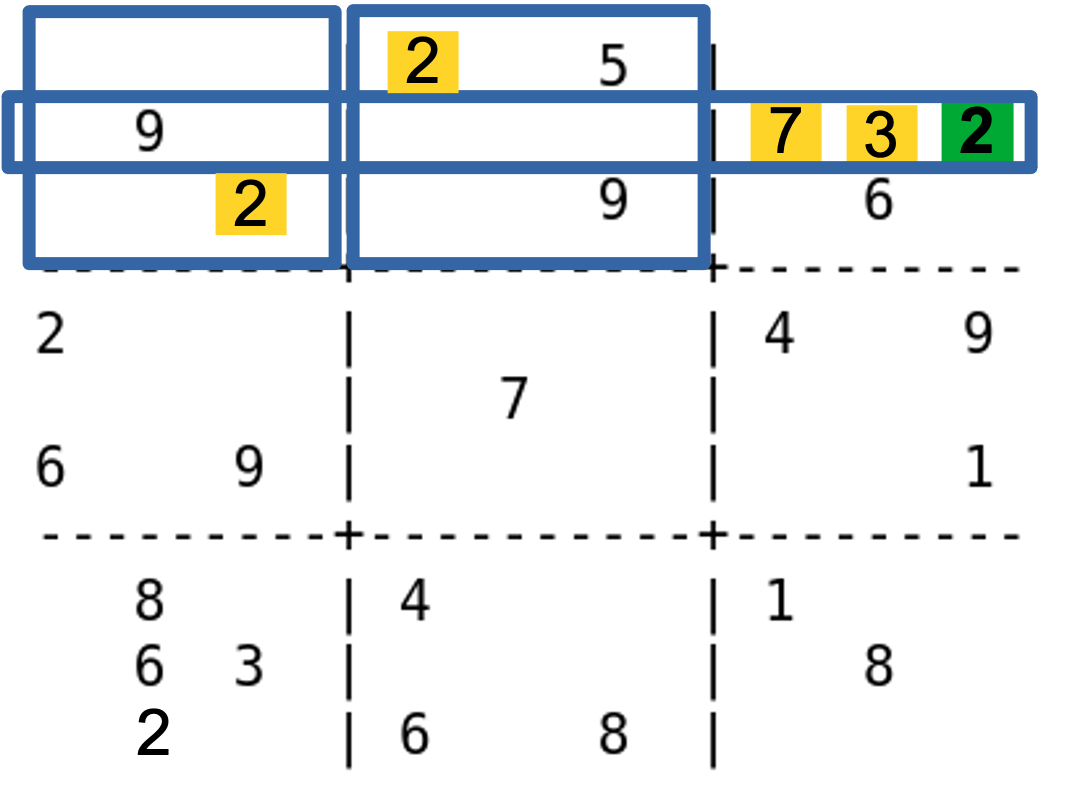
\includegraphics[width=\textwidth]{figures/sudoku_sequence/sudoku-step2}
		\end{minipage}\hfill \pause
		or \hfill
		\begin{minipage}{0.30\textwidth}
			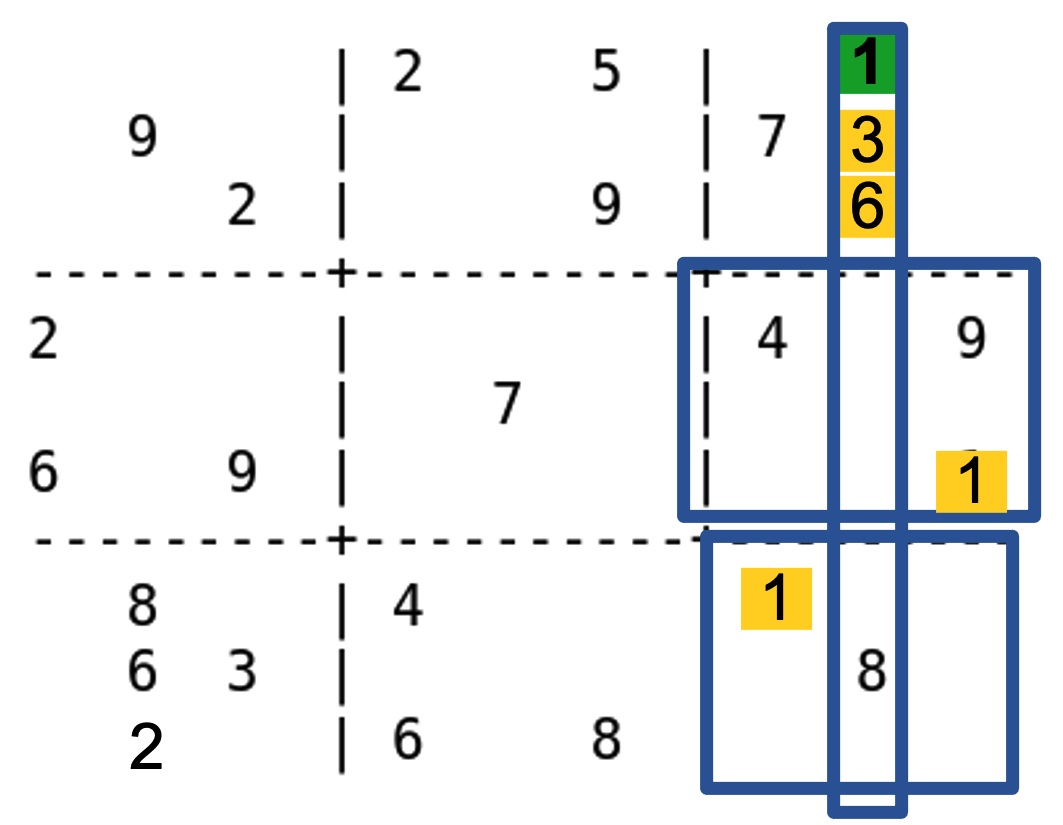
\includegraphics[width=\textwidth]{figures/sudoku_sequence/sudoku-step3bis}
		\end{minipage}
	\end{frame}	
	
	
	\begin{frame}
%		\frametitle{Stepwise explanations for CSPs}
		\frametitle{The best/easiest explanation step...}
%		\begin{center} 
			\textbf{What is a \emph{good} explanation ?} \pause \\
			
			Let $\mathbf{f}  ($ 
\includegraphics[width=10pt]{figures/explanation_steps/explanation_E}, {
\includegraphics[width=10pt]{figures/explanation_steps/explanation_S}}, {
\includegraphics[width=10pt]{figures/explanation_steps/explanation_N}} $)$ be a cost-function that quantifies how good (e.g. easy to understand) an explanation step is.
			\pause 
		
		\vspace*{1cm}
		
\textbf{What is the \emph{best/easiest} explanation step? }\pause
				\begin{algorithm}[H]

							$X_{best} \gets \mathit{nil}$\;\pause
							\For{\color{black} {
\includegraphics[width=10pt]{figures/explanation_steps/explanation_N}} $\in$ \texttt{propagate({
\includegraphics[width=10pt]{figures/explanation_steps/explanation_S_full}})}}{
										
										$X \gets \mathtt{{MUS}}($ 
\includegraphics[width=10pt]{figures/explanation_steps/explanation_E_full} $\&$ {
\includegraphics[width=10pt]{figures/explanation_steps/explanation_S_full}} $\& \lnot$ {
\includegraphics[width=10pt]{figures/explanation_steps/explanation_N}} $)$\;\pause
										\uIf{$f(X)<f(X_{best})$}{
												$X_{best} \gets X$\;
											}
									}
								\Return{$X_{best}$} 
							\end{algorithm}
			

%		\end{center}
	\end{frame}
	
	\begin{frame}{Motivation}
	\framesubtitle{Challenges and open questions from \cite{bogaerts2020step}}
	
	\begin{minipage}{0.53\textwidth}
		%\begin{description}%[font=\color{vuborange}\itshape]
		%	\item[Optimality] Explanations not provably optimal, \emph{heuristically} found.
		%\end{description}

		\begin{itemize}
			\item[Q1] \emph{\textbf{Optimality}} w.r.t $\mathbf{f}$
			\item[$\triangleright$] MUS guarantees non-redundancy but ... not optimality.
			%				\item MUS-based heuristic
			\item[$\triangleright$] Alternative: SMUS $\#$-minimal (\cite{ignatiev2015smallest})
		\end{itemize} 
		\only<2->{				Explanation generation takes a lot of time: 
			\only<3->{
		\begin{itemize}
					\item[Q2] Can we \emph{avoid looping over the literals} when searching for the next best explanation ?
					\only<4->{\item[Q3] Can we \emph{reuse information} from an explanation call to another?}
				\end{itemize}}}
		%\end{description}
	\end{minipage}
\hfill
	\begin{minipage}{0.42\textwidth}

			\begin{algorithm}[H]
				
				{\color{gray} \small $X_{best} \gets \mathit{nil}$\;
					\For{\color{gray} \only<3>{\color{vuborange}} n  $\in$ \texttt{propagate($C$)}}{
						
						{\color{gray}\only<1>{\color{vuborange}}$X \gets \call{MUS}{(C \land E \land \neg n)}$}\;
						\uIf{\color{gray}\only<1>{\color{vuborange}} $f(X)<f(X_{best})$}{
							{\color{gray}\only<1>{\color{vuborange}}$X_{best} \gets X$}\;
						}
					}
					\Return{\color{gray}\only<1>{\color{vuborange}} $X_{best}$} }
%				\caption{Explain 1 step}
			\end{algorithm}
		
	\end{minipage}
	
	%		\end{center}


\end{frame}
	
	
	
	
	\section{The OCUS Problem}
	
	 \begin{frame}
		\tableofcontents[currentsection]
	\end{frame}			
	
			\begin{frame}{OCUS-Based explanation generation}
			\framesubtitle{The OCUS\footnote{Optimal \emph{Constrained} Unsatisfiable Subset} problem}
			\begin{definition}
				\small
				Let $\formula$ be a formula, $f:2^{\formula} \to \nat$ a cost function and  $p$ a predicate $p: 2^{\formula}\to \{\ltrue,\lfalse\}$. We call %a set $U\subseteq \formulag$ a \emph{$p$-constrained $f$-OUS} of \formulag ($(p,f)$-OUS) \tias{what with the OCUS name here?} \bart{I propsoe to say. We call 
					$\subsetT \subseteq \formula$ an \emph{OCUS}  of \formula (with respect to $f$ and $p$) if \begin{itemize}                                      
						\item $\subsetT$ is unsatisfiable,
						\item $p(\subsetT)$ is true
						\item \emph{all other unsatisfiable $\subsetT'\subseteq \formula$ with $p(\subsetT')=\ltrue$ satisfy $f(\subsetT')\geq f(\subsetT)$}.
					\end{itemize}
				\end{definition} \pause
				
				\vfill
				Applied to explanation generation: \pause
				\begin{itemize}
					\item[Q1] \textit{\emph{(Optimality)}} {\color{red}$f$} ensures finding `best' explanation \pause
					\item[Q2] \textit{\emph{(Looping)}} {\color{red}$p$} allows formulating explaining 1 literal at a time using an extra constraint
				\end{itemize}
							
			\end{frame}		
			
			
			\newcommand\onestepo{\ensuremath{\call{explain-One-Step-ocus}}\xspace}
			\begin{frame}{OCUS-Based explanation generation}

					\hspace{0.3\textwidth}
					\begin{minipage}{0.5\textwidth}
					\begin{algorithm}[H]
					$X_{best} \gets \mathit{nil}$\;
						\For{\color{black}n  $\in$ \texttt{propagate($C$)}}{
							
							$X \gets \call{MUS}{(C \land E \land \neg n)}$\;
							\uIf{\color{black} $f(X)<f(X_{best})$}{
								$X_{best} \gets X$\;
							}
						}
						\Return{\color{black}$X_{best}$} 
				\end{algorithm}
					\end{minipage} \pause

			\[\downarrow\]


									\hspace{0.09\textwidth} \begin{minipage}{0.9\textwidth}				
				\begin{algorithm}[H]
					\DontPrintSemicolon
					$p \leftarrow$ \texttt{exactly-one}$(\{ \lnot$ {
\includegraphics[width=10pt]{figures/explanation_steps/explanation_N}} $ | $ {
\includegraphics[width=10pt]{figures/explanation_steps/explanation_N}} $ \in \LitsToExplain\})$\;
					{\Large $\emph{\mathtt{{OCUS}}}($}{\large 
\includegraphics[width=10pt]{figures/explanation_steps/explanation_S_full} $\wedge$ {
\includegraphics[width=10pt]{figures/explanation_steps/explanation_E_full}} $\wedge \{ \lnot$ {
\includegraphics[width=10pt]{figures/explanation_steps/explanation_N}} $ | $ {
\includegraphics[width=10pt]{figures/explanation_steps/explanation_N}} $ \in \LitsToExplain\}, \emph{\mathbf{f}}, \emph{\mathbf{p}})$ } \;
%					$\call{OCUS}(S \wedge E \wedge \{\lnot n \ | \ n \in \LitsToExplain\}, \emph{f, p})$\;
				\end{algorithm}
								\end{minipage}

				
			\end{frame}


%			\section{An OCUS algorithm: A hitting set-based algorithm}
%
%						\begin{frame}{Background and notation}
%				\framesubtitle{Minimum Correction Subset vs Satisfiable Subsets}
%				
%				\only<1->{ Consider unsatisfiable  CNF $\formula$ over atoms $x_1, x_2$:}
%				\only<2>{\[ c_1 := \lnot x_1 \vee \lnot x_2  \qquad  c_2 := \lnot x_1 \vee  x_2 \qquad c_3 := \lnot x_2  \qquad  c_4 := x_1\]}
%				
%				\only<3>{\[ \emph{c_1 := \lnot x_1 \vee \lnot x_2  \qquad  c_2 := \lnot x_1 \vee  x_2 }  {\color{blue}\qquad c_3 := \lnot x_2  \qquad  c_4 := x_1}\]}
%				
%				\only<4>{\[ c_1 := \lnot x_1 \vee \lnot x_2  \qquad  c_2 := \lnot x_1 \vee  x_2  \qquad c_3 := \lnot x_2  \qquad  \emph{   c_4 := x_1} \]}
%				\only<3->{	\begin{definition}
%						A set $C \subseteq \formula $ is a \only<3>{\emph{correction subset}}\only<4->{correction subset} of $\formula$ if \only<3>{{\color{blue} $ \formula \setminus \subsetT$}}\only<4->{ $ \formula \setminus \subsetT$} is satisfiable, a.k.a. {\only<3>{\color{blue}} satisfiable subset.} \\
%						\only<4->{A correction set $\subsetT$ is a \emph{minimum correction subset} if no strict subset $\subsetT' \subset \subsetT$ is also a correction set.}
%				\end{definition} }
%			\end{frame}



			
					\begin{frame}{An OCUS algorithm: A hitting set-based algorithm}
				\framesubtitle{Implicit Hitting set duality}
				
				\begin{itemize}
					\item[$\triangleright$] Exploit implicit hitting set--based duality between {\color{blue}MCSes} and {\color{teal}MUSes} (\cite{DBLP:journals/jar/LiffitonS08,ai/Reiter87})
				\end{itemize}\pause
				
				\begin{theorem}\label{prop:MCS-MUS-hittingset}
					%     
					A set  $\subsetT \subseteq \formula$ is a MCS of $ \formula$ iff  it is a \emph{minimum hitting set} of \muses{\formula}. \\
					A set  $\subsetT \subseteq \formula$ is a MUS of $ \formula$ iff  it is a \emph{minimum hitting set} of \mcses{\formula}.
				\end{theorem} \pause
				\begin{itemize}
					\item[$\triangleright$] Extend this to OCUS:
				\begin{itemize}	
				\item Compute \emph{optimal} hitting sets \pause
				\item Impose \emph{constraint} on the hitting sets
			\end{itemize}
				\end{itemize}
				
			\end{frame}
			
			
			
			\subsection{Optimal Hitting set problem}
				
\begin{frame}
	\tableofcontents[currentsubsection]
\end{frame}			
				\begin{frame}{\emph{Optimal} Hitting set problem}
					\pause
					\begin{itemize}
						\item Set of elements (i.e. constraints) $\{c_1,c_2,...,c_n\}$
						\item Collection $\m{H}$ of sets-to-hit  (i.e.~subsets of the set of elements)\pause
						\item cost associated for every element:\\
						 \hspace*{2cm}$w_1 =  \emph{3}, w_2= \emph{5}, w_3 = w_4 = ...= w_8 = 1$\pause \vfill
						\item[\textbf{Goal}] Find an \emph{optimal} hitting set such that every set-to-hit is hit by at least once an element of the hitting set with \emph{minimal total cost}.
					\end{itemize} \pause
					\vfill
					\begin{minipage}{0.48\textwidth}
						For example: 
						\begin{enumerate}
							\item[$H_1$] = {\only<5>{\color{blue}}$\{c_3, c_5\}$}
							\item[$H_2$] = {\only<6>{\color{blue}}$\{c_2, c_4, c_7\}$}
							\item[$H_3$] = {\only<7>{\color{blue}}$\{c_2, c_6\}$}
							\item[$H_4$] = {\only<8>{\color{blue}}$\{c_1, c_8\}$}
						\end{enumerate}
					\end{minipage}
					\begin{minipage}{0.48\textwidth}
						Optimal hitting sets:
						\begin{itemize}
							\item $\{\only<5->{{\color{blue}c_3},} \only<6->{{\color{blue}c_4},} \only<7->{{\color{blue}c_6},} \only<8->{{\color{blue}c_8}}\}$ \only<9>{\emph{\checkmark}
							\begin{itemize}
								\item cost: \emph{4}
							\end{itemize}}
							\only<10>{\item {$\{c_1, c_2, c_3\}$}
							\begin{itemize}
								\item cost: \emph{7}
							\end{itemize}
							\item \dots}
						\end{itemize}
					\end{minipage}
				\end{frame}
			
			

%

		
%			\begin{frame}{An OCUS algorithm: A hitting set-based algorithm}
%				\framesubtitle{\cite{ijcai2021-191}}
%				\pause
%				
%				
%					\begin{algorithm}[H]
%						\caption{$\comus(\formula,f,p)$ } \label{alg:comus}\vspace*{-0.3cm}
%						\DontPrintSemicolon
%						$\setstohit  \gets \emptyset$ \tcp*{ Collection of sets-to-hit} \pause
%						\While{\color{black} true}{
%							$\subsetT \gets \emph{\cohs(\setstohit,f,p)} $ \; \pause
%							\If{\color{black} $\lnot \sat(\subsetT)$}{
%								\Return{\color{black}$\subsetT$} \tcp*{ OCUS found!}\pause
%							}
%							$\setstohit  \gets \setstohit \ \cup $ 				{\color{blue}$\corrss(\subsetT,\formula)$} 
%						}
%					\end{algorithm}
%				\end{frame}

\subsection{The algorithm}
\begin{frame}
	\tableofcontents[currentsubsection]
\end{frame}			
	\begin{frame}{OCUS: An efficient game of Ping-Pong}
	\only<1>{
		\begin{figure}
			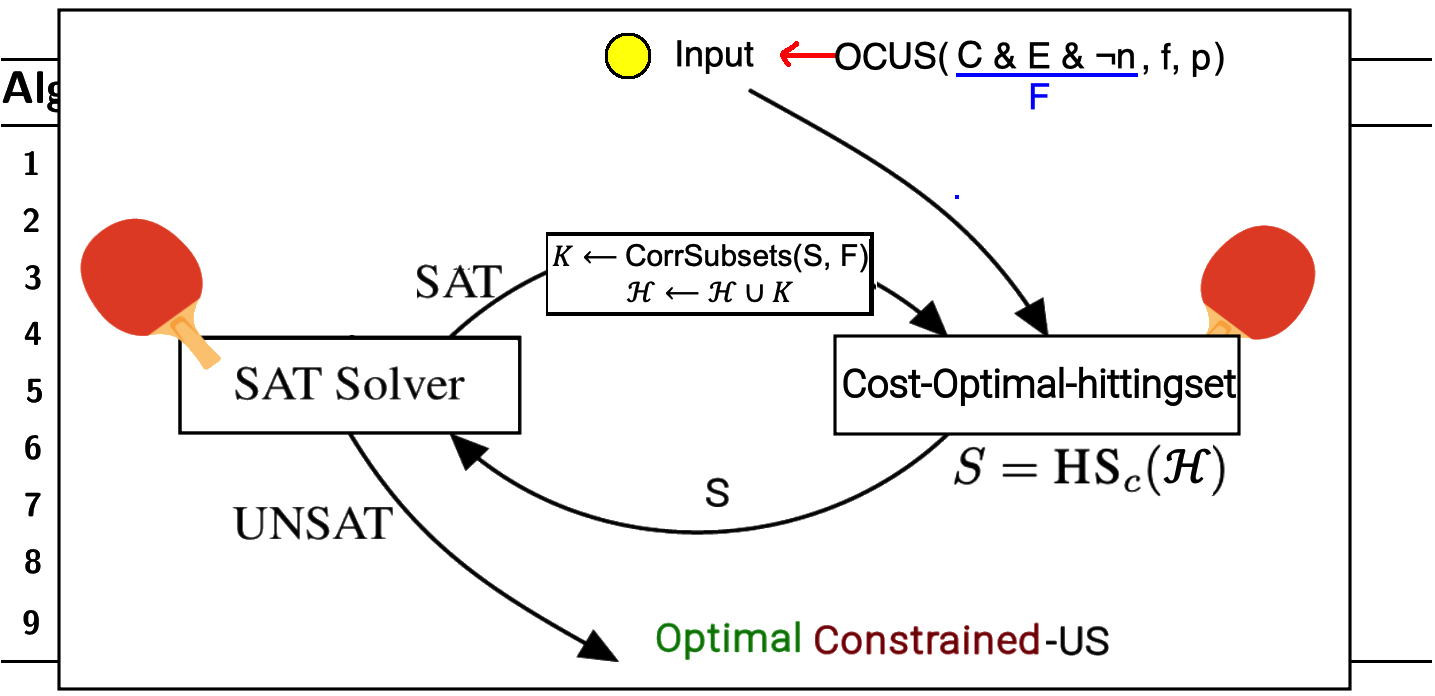
\includegraphics[width=\textwidth]{figures/ping_pong/algo_with_ping_pong_0.png}
		\end{figure}
	}
	\only<2>{
		\begin{figure}
			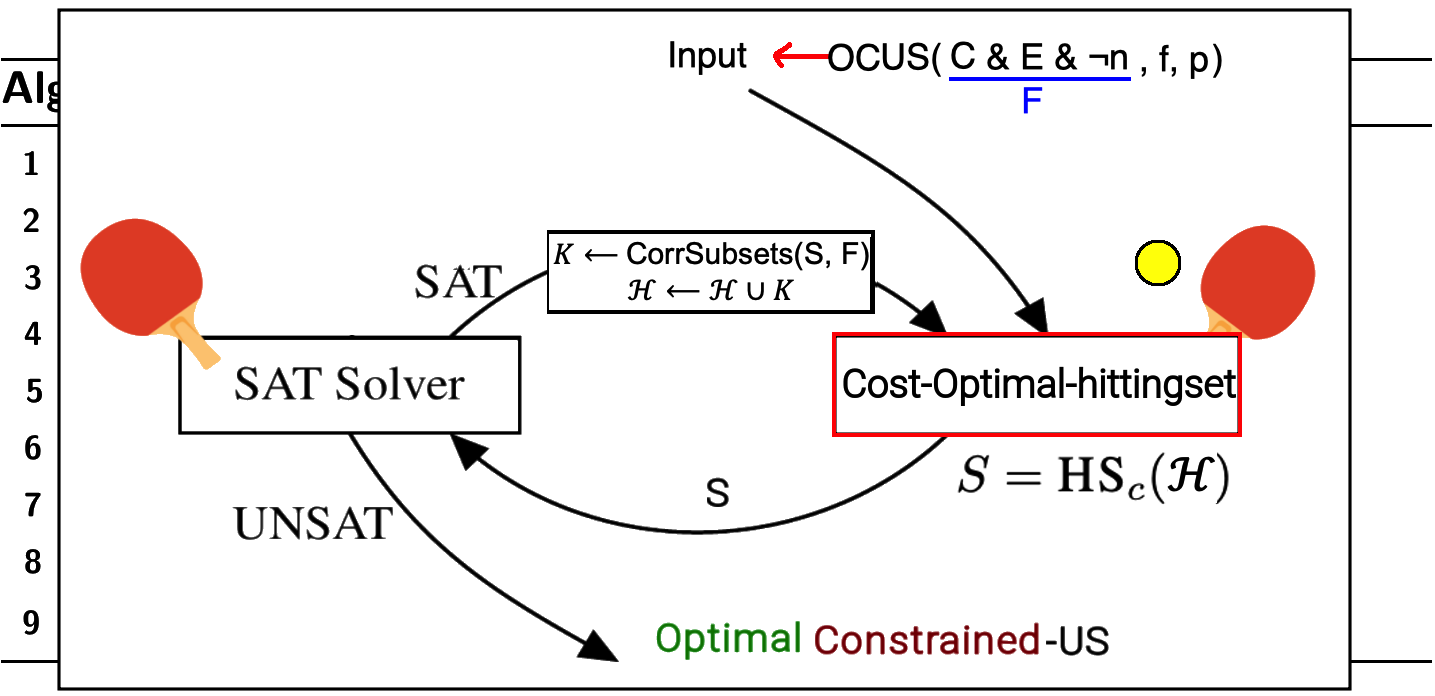
\includegraphics[width=\textwidth]{figures/ping_pong/algo_with_ping_pong.png}
		\end{figure}
	}
	\only<3>{
		\begin{figure}
			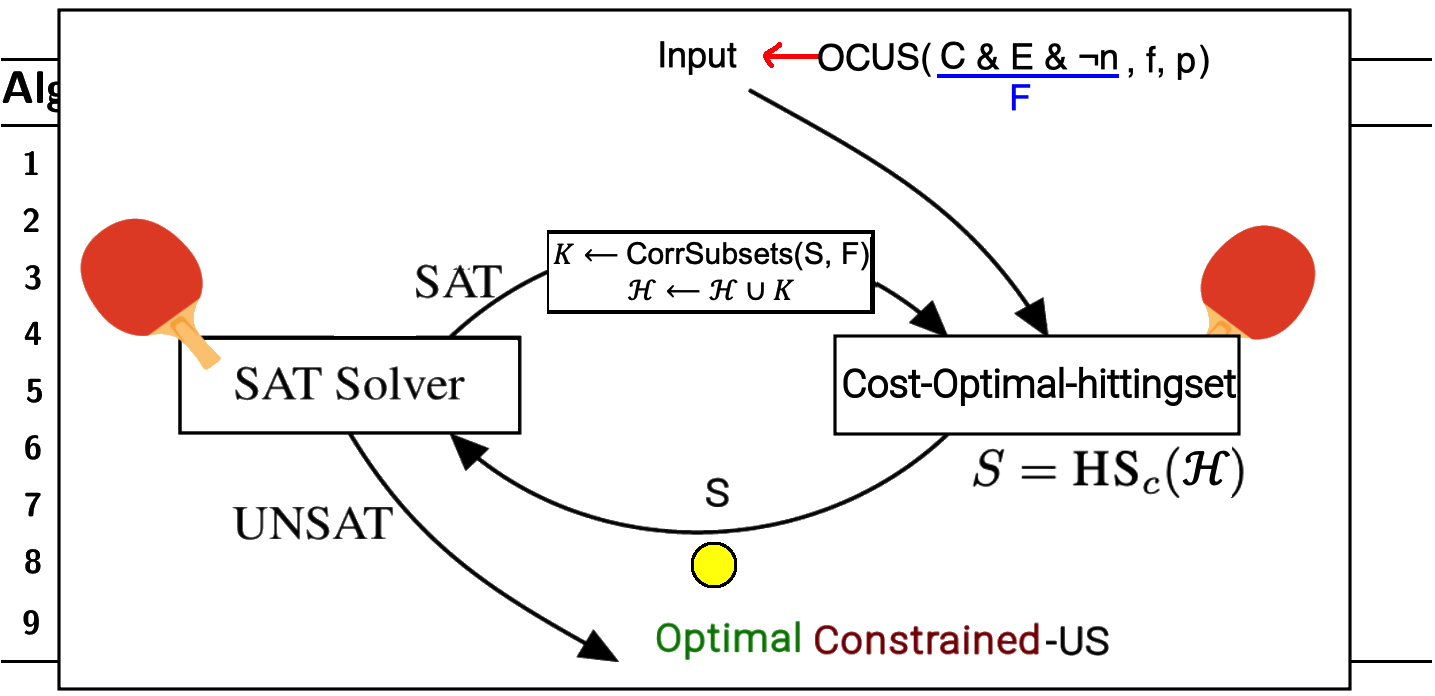
\includegraphics[width=\textwidth]{figures/ping_pong/algo_with_ping_pong1.png}
		\end{figure}
	}
	\only<4>{
		\begin{figure}
			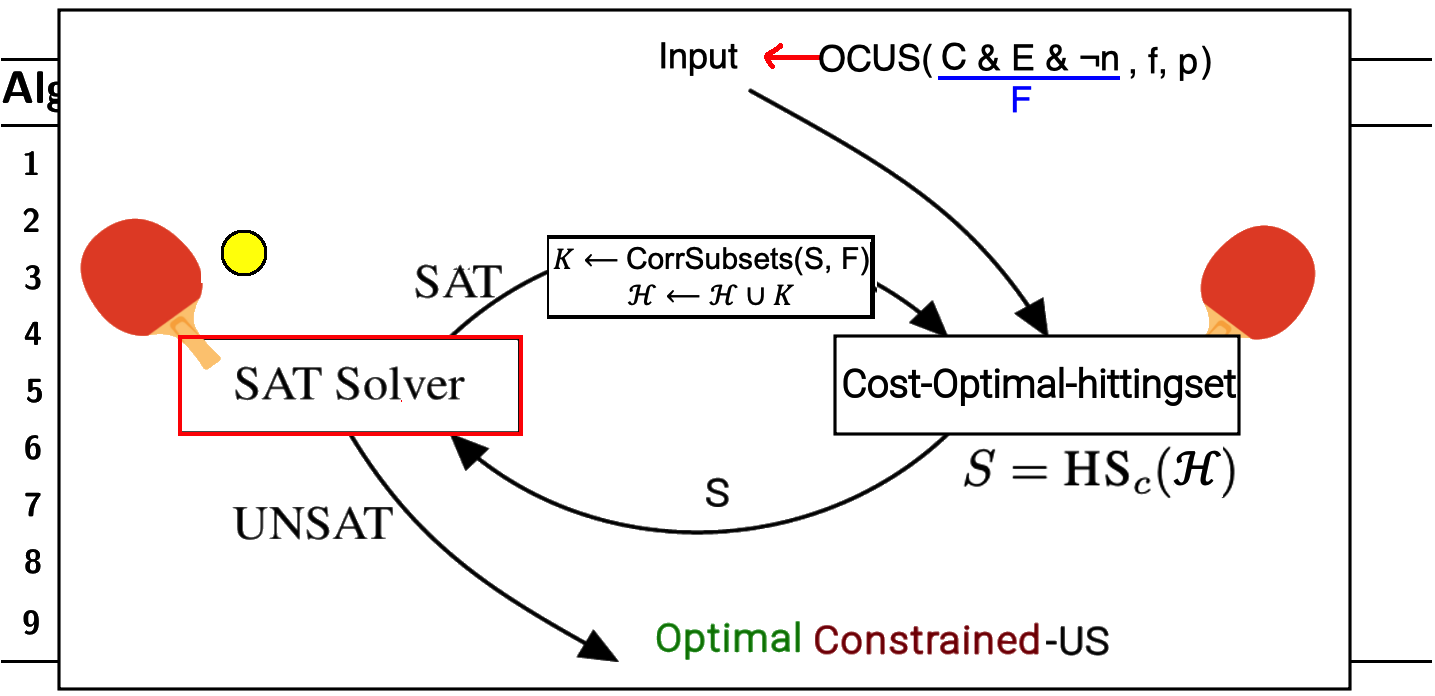
\includegraphics[width=\textwidth]{figures/ping_pong/algo_with_ping_pong2.png}
		\end{figure}
	}
	\only<5>{
		\begin{figure}
			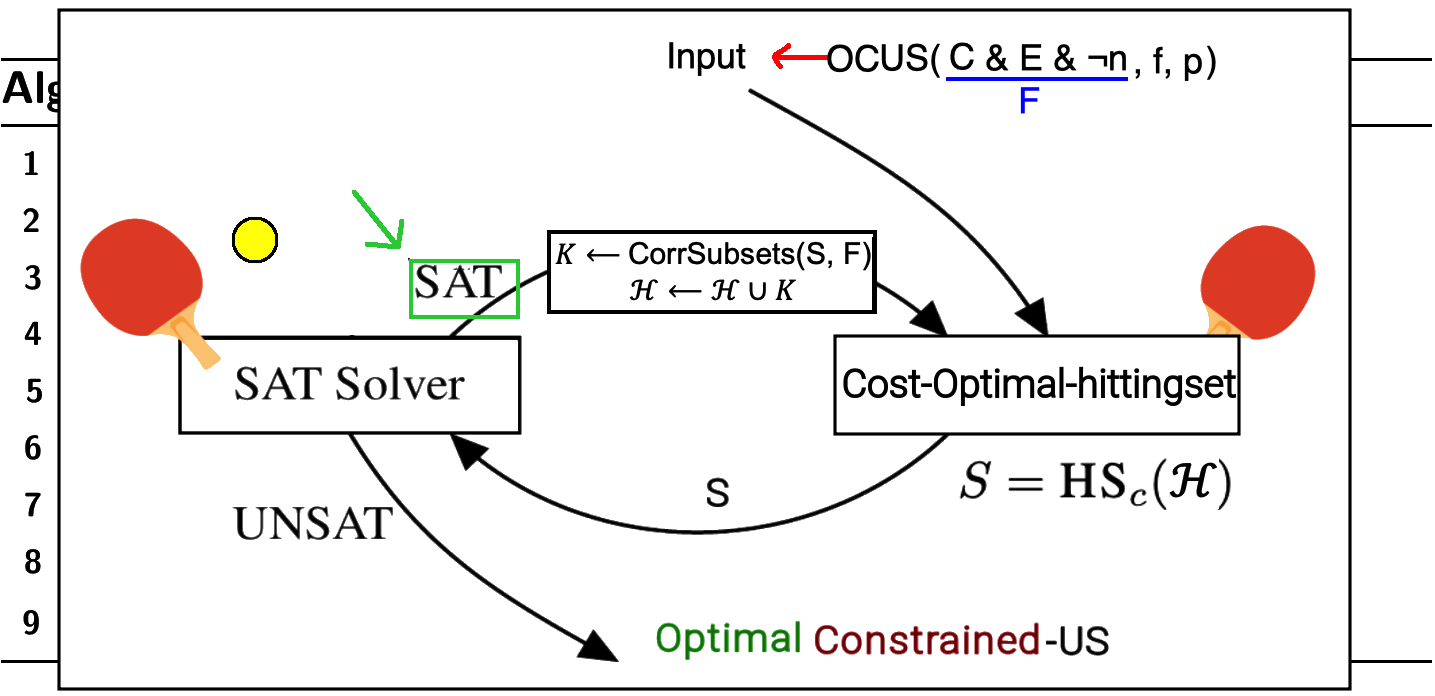
\includegraphics[width=\textwidth]{figures/ping_pong/algo_with_ping_pong2a.png}
		\end{figure}
	}
	\only<6>{
		\begin{figure}
			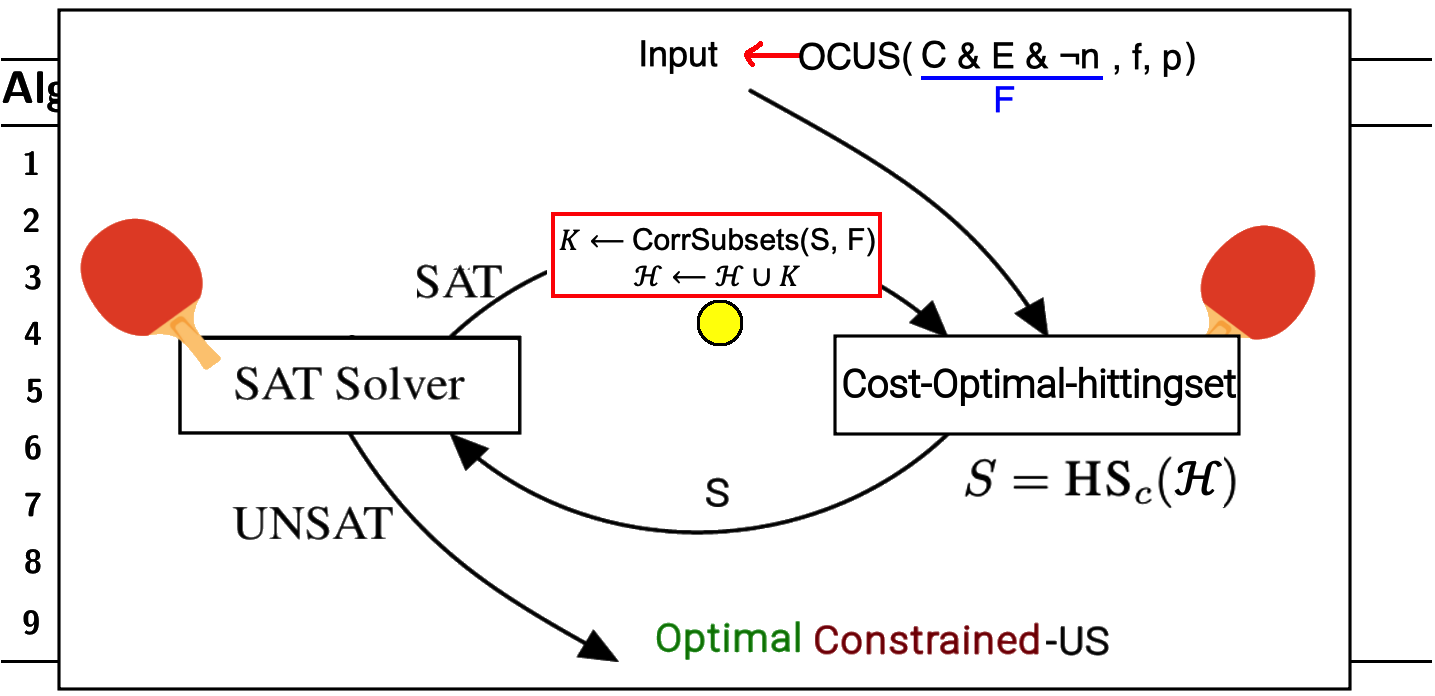
\includegraphics[width=\textwidth]{figures/ping_pong/algo_with_ping_pong2b.png}
		\end{figure}
	}
	\only<7>{
		\begin{figure}
			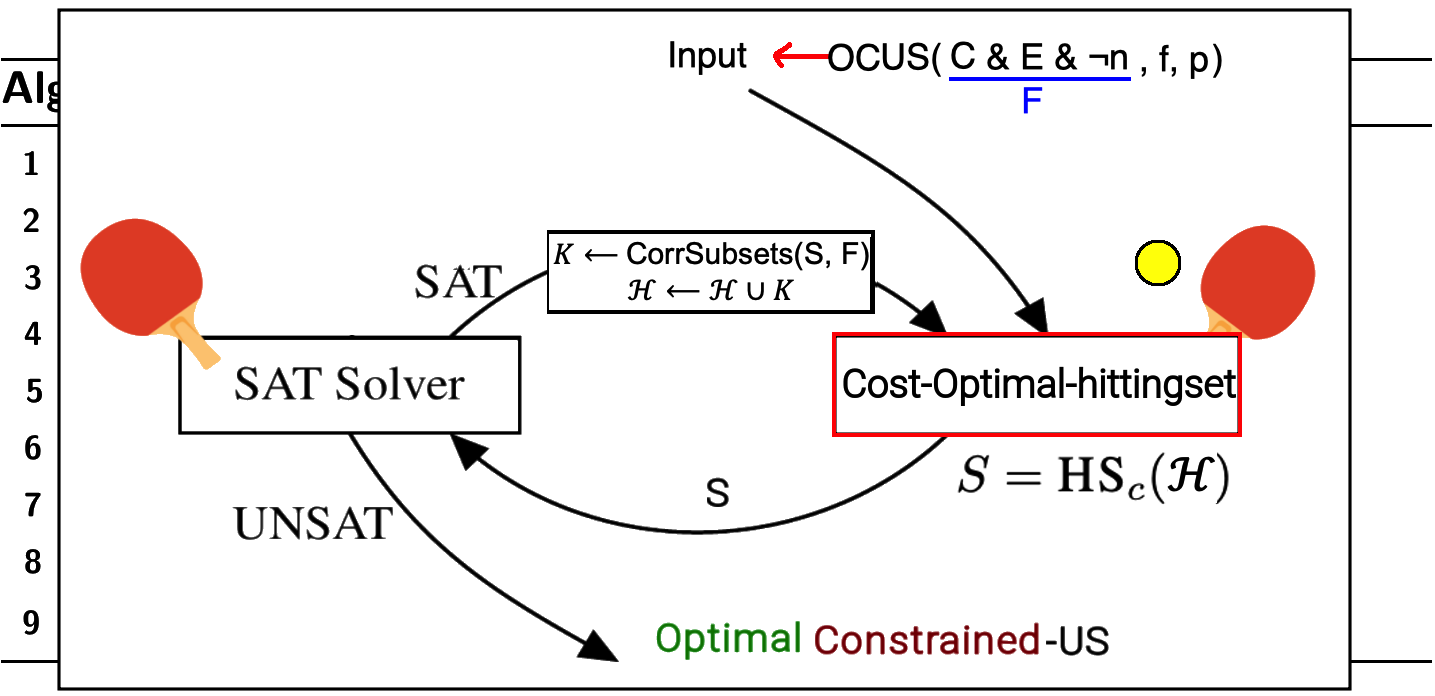
\includegraphics[width=\textwidth]{figures/ping_pong/algo_with_ping_pong.png}
		\end{figure}
	}
	
	\only<8>{
		\begin{figure}
			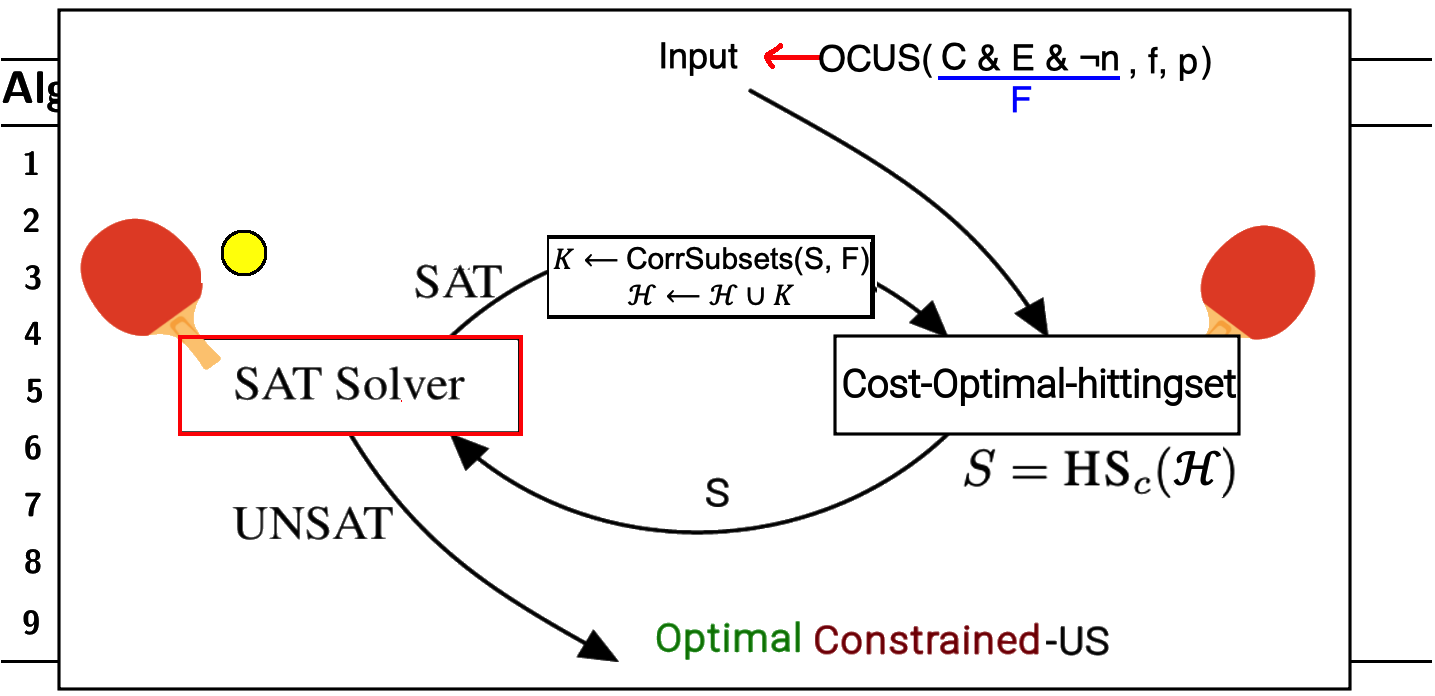
\includegraphics[width=\textwidth]{figures/ping_pong/algo_with_ping_pong2.png}
		\end{figure}
	}
	\only<9>{
		\begin{figure}
			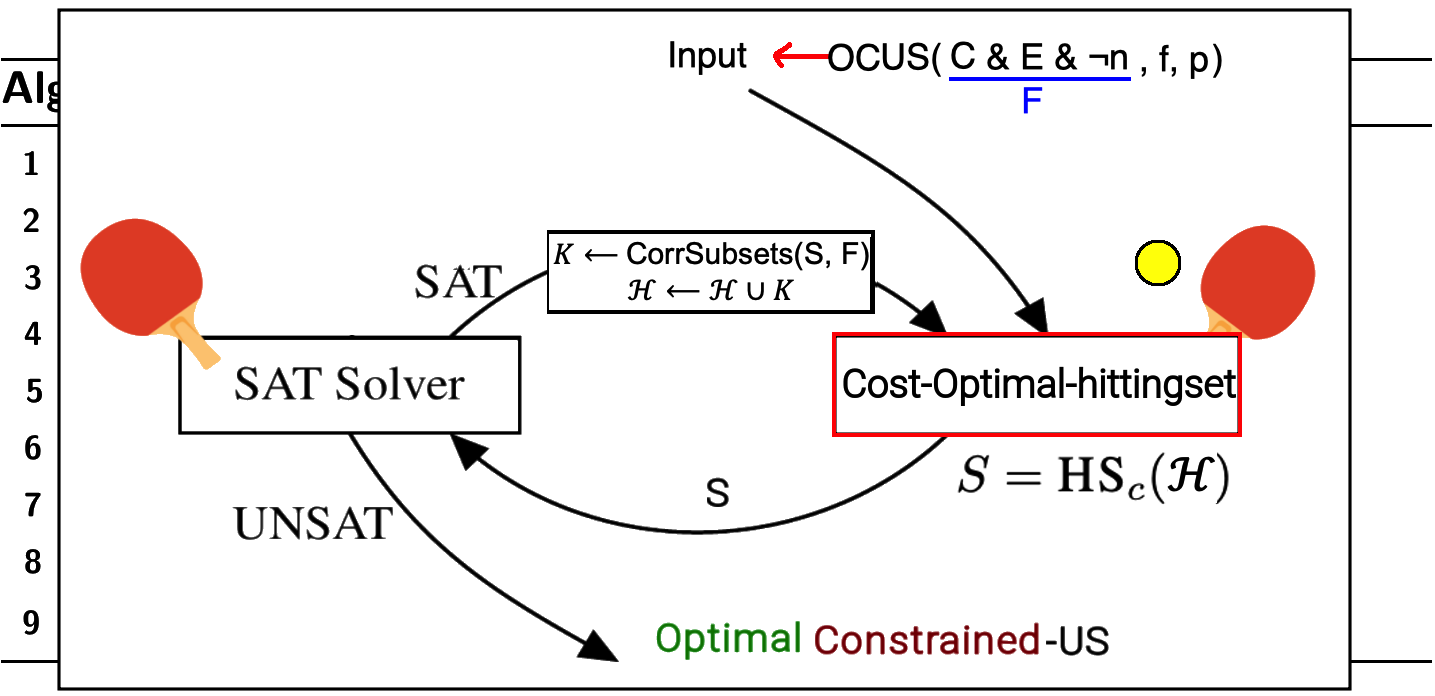
\includegraphics[width=\textwidth]{figures/ping_pong/algo_with_ping_pong.png}
		\end{figure}
	}
	
	\only<10>{
		\begin{figure}
			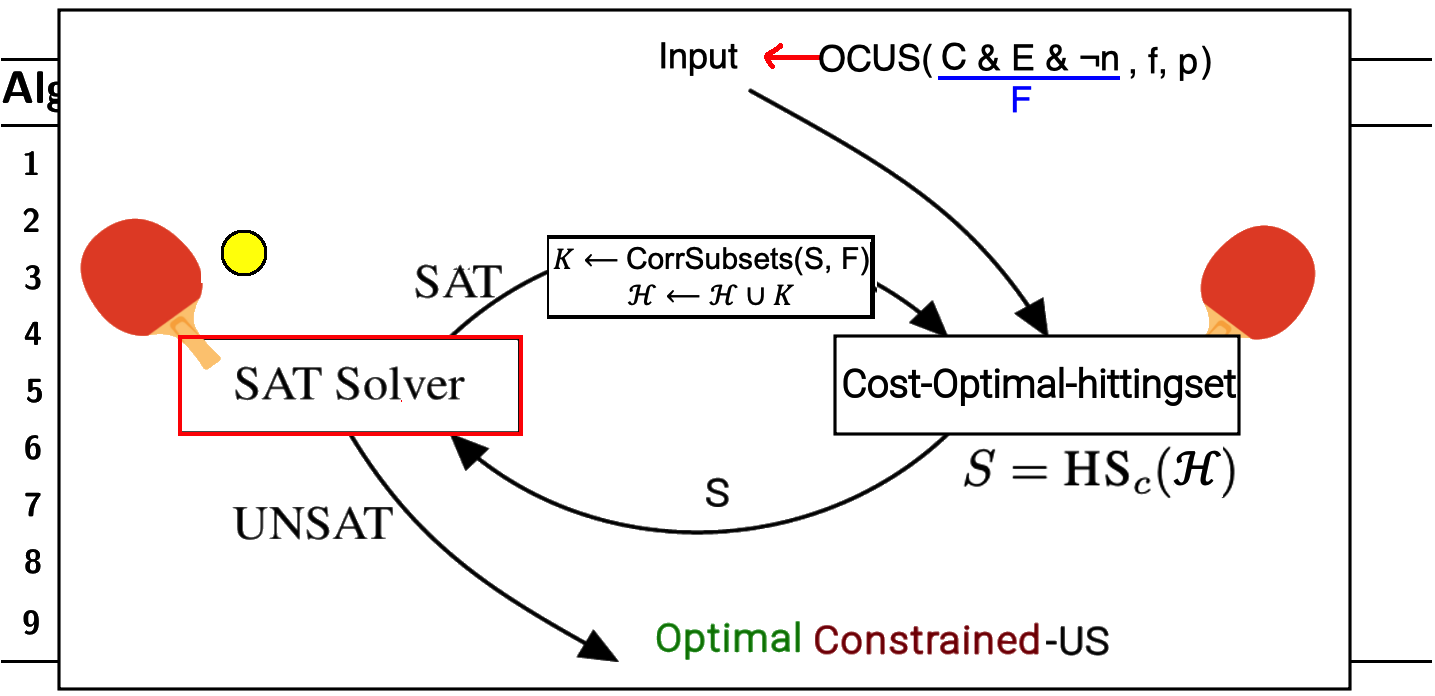
\includegraphics[width=\textwidth]{figures/ping_pong/algo_with_ping_pong2.png}
		\end{figure}
	}
	\only<11>{
		\begin{figure}
			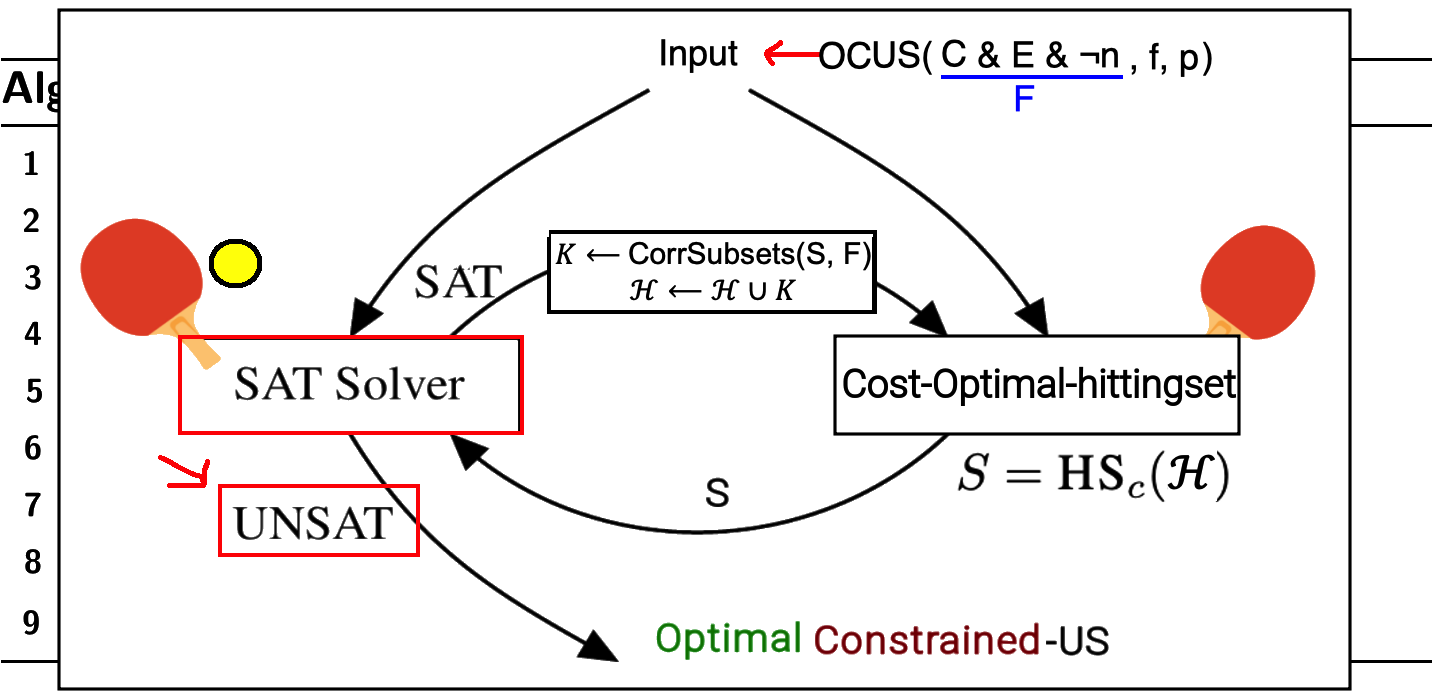
\includegraphics[width=\textwidth]{figures/ping_pong/algo_with_ping_pong_2c.png}
		\end{figure}
	}
	\only<12>{
		\begin{figure}
			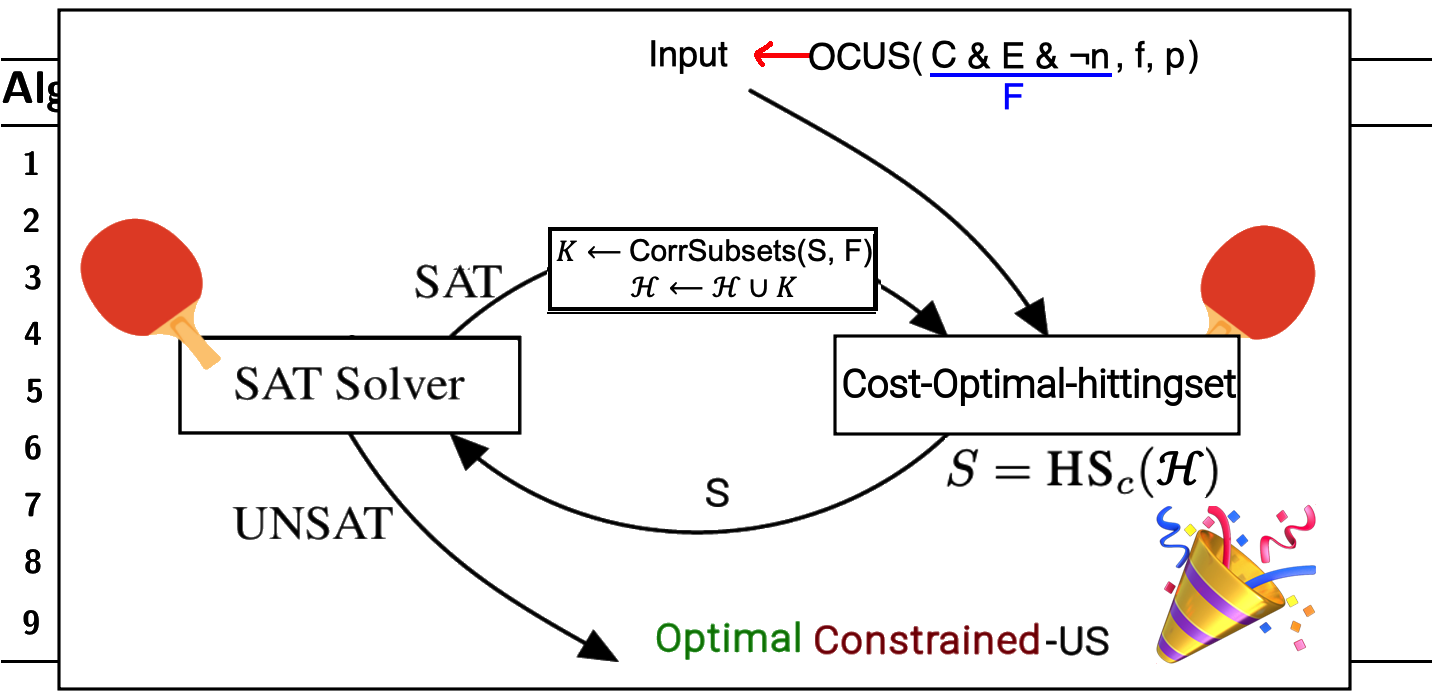
\includegraphics[width=\textwidth]{figures/ping_pong/algo_with_ping_pong3.png}
		\end{figure}
		{\tiny \url{https://flyclipart.com/party-popper-emoji-on-apple-ios-celebration-emoji-png-610281}}
	}
	\newcommand\hitset{\m{\mathcal{H}}}
	
	%\begin{frame}{Correctness}
	%	\begin{theorem}\label{thm:soundcomplete}
		%		Let $\hitset$ be a set of correction subsets of \formula. 
		%		If $\subsetT$ is a hitting set of \hitset that is $f$-optimal among the hitting sets of \hitset satisfying a predicate $p$, and  $\subsetT$ is unsatisfiable, then $\subsetT$ is an OCUS of \formula. 
		%		
		%		If  $\hitset$ has no hitting sets satisfying $p$, then $\formula$ has no OCUSs.
		%	\end{theorem}
\end{frame}

%				\begin{frame}
%				\begin{center}
%				\Large
%				\textbf{Q}: How do I \emph{efficiently} compute OCUSs?				
%			\end{center}
%\end{frame}


				\begin{frame}
					\frametitle{How do I \emph{efficiently} compute OCUSs?}
	\only<1>{
		\begin{figure}
		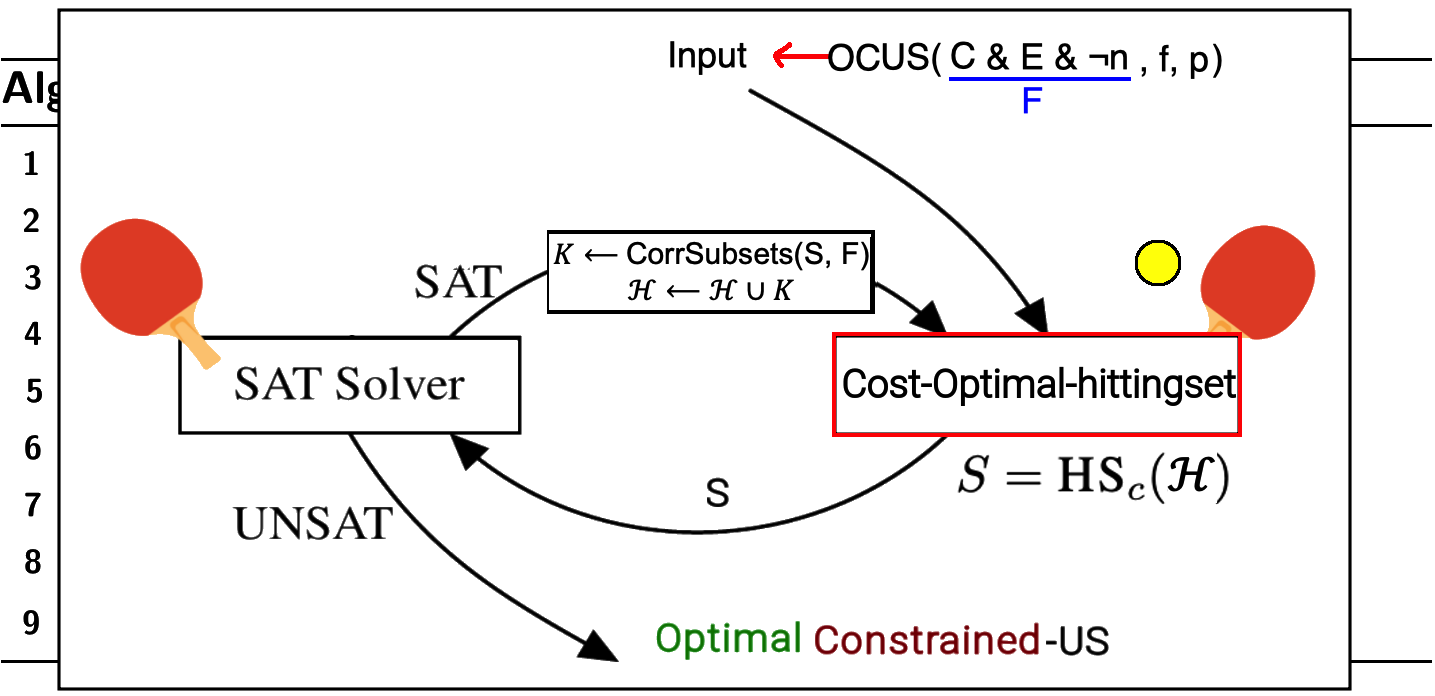
\includegraphics[width=0.7\textwidth]{figures/ping_pong/algo_with_ping_pong.png}
	\end{figure}
\vspace{90pt}}
	\only<2->{
		\begin{figure}
			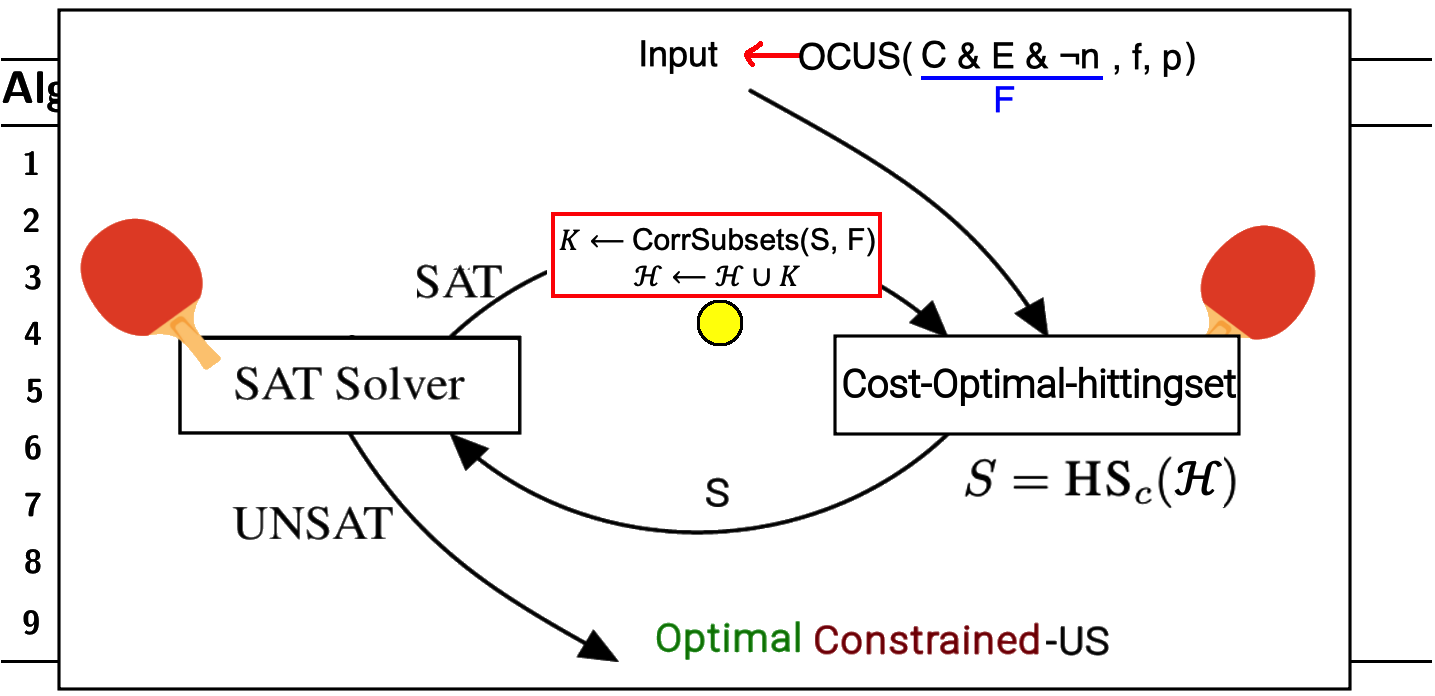
\includegraphics[width=0.7\textwidth]{figures/ping_pong/algo_with_ping_pong2b.png}
		\end{figure}
%			\textbf{OCUS}
%			\begin{itemize}
%				\item Take advantage of the strengths of each solver: 
%				\begin{itemize}
%					\item[MIP] Efficient at solving the hitting set problem \pause
%					\item[SAT] Oracle for checking satisfiability \pause
%				\end{itemize}
%				\item Time spent in checking satisfiability is negligible \pause
%				\item Most time (~96\%) is spent in computing opt.~hitting sets \pause
%				\item Calls to the hitting set solver become more difficult as the collection of sets-to-hit expands\pause
%				\begin{itemize}
%				\item[$\rightarrow$] Shift the computation towards extracting \emph{better} correction subsets
%				\end{itemize}
%			\end{itemize}

				{\color{blue}$\corrss(\subsetT,\formula)$} 
				\begin{itemize}
					\item $\{  \formula \setminus \subsetT\}$ \pause
					\item   $\{  \formula \setminus \grow(\subsetT, \formula)\}$  \pause 
			\begin{itemize}
				\item[$\rightarrow$] \textit{efficient} vs \textit{qualitative} grow ? \pause
					\item[$\rightarrow$] MaxSAT vs SAT-based heuristic\pause
				\end{itemize}
					\item Multiple \textit{disjoint} correction subsets ? 
				\end{itemize}}

			\end{frame}
%						\begin{frame}
%		\frametitle{Splitting OCUS-calls}
%				%\end{minipage}
%							\vfill
%				\begin{center}\Large
%				Did we go too generic ?					
%				\end{center}\pause
%			\vfill
%				By making OCUS `generic' (1 OCUS-call to explain 1 literal), we introduce \emph{overhead}.  \pause
%					\begin{itemize}
%						\item[$\rightarrow$] At every explanation step, OCUS computes intermediate hitting sets containing literals that might not lead to an cost-optimal explanation.
%						\item[$\rightarrow$] Compute OCUS only for the most promising literal ?
%					\end{itemize}
%							\vfill
%%				\end{itemize}
%			\end{frame}
%\begin{frame}
%	\frametitle{Splitting OCUS-calls}
%		\begin{figure}
%	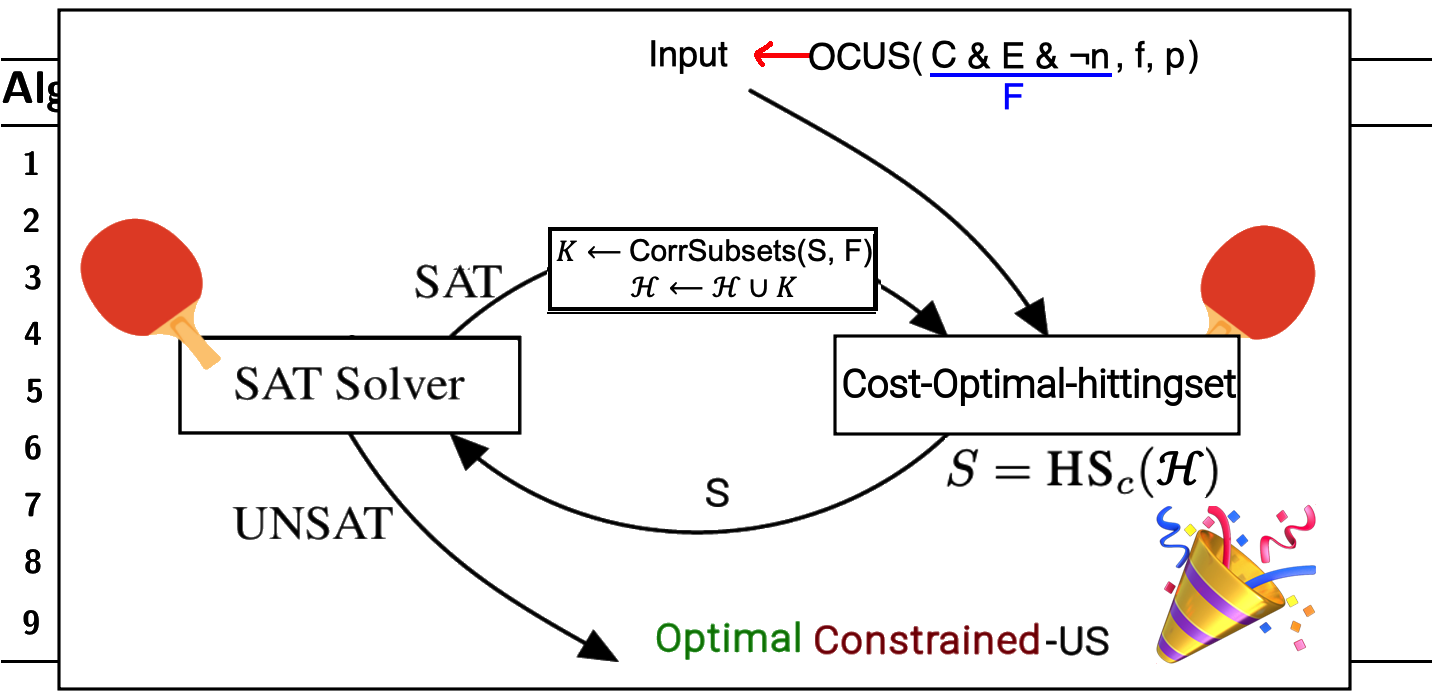
\includegraphics[width=0.5\textwidth]{figures/ping_pong/algo_with_ping_pong3.png}
%\end{figure}
%{\small
%\begin{algorithm}[H]
%	\DontPrintSemicolon
%	$queue \gets$ \texttt{InitializePriorityQueue($(\ell, \emptyset,\emptyset): 0 \ | \ \forall \ell \in E_{end} \setminus E$)}\; \pause
%	\While{$(\ell, \m{S}_\ell, \setstohit_{\ell}) \gets queue.pop()$}{\pause
%			\If{\color{black}$\lnot \sat(\m{S}_\ell)$}{
%				\Return{\color{black}$\m{S}_\ell$} 
%			}
%			$\m{K} \gets \corrss(\subsetT_\ell, (\formulac \land E \land \neg \ell))$\;
%			$\setstohit_\ell  \gets \setstohit_\ell  \cup \m{K} $\;
%			$\m{S}_\ell \gets OptHittingSet(\setstohit_\ell,f) $  \;
%			\texttt{queue.push($(\ell, \m{S}_\ell, \setstohit_{\ell}): f(\m{S_\ell})$)}\;
%		}
%	\end{algorithm}}
%
%			\end{frame}
			
			
			\section{Open questions and challenges}
			
			 \begin{frame}
				\tableofcontents[currentsection]
			\end{frame}			
			
						\begin{frame}{Improving efficiency of the OCUS algorithm..}
				\framesubtitle{...in the context of explanation sequence generation}
							\begin{center}
	\large
	Can we \emph{improve} OCUS-calls in the context of explanation \emph{sequence} generation?
\end{center}
			\end{frame}
		
						\begin{frame}{Improving efficiency of the OCUS algorithm..}
			\framesubtitle{...in the context of explanation sequence generation}
			
			\textbf{Incrementality}
			\begin{itemize}
				\item Can we re-use of information between explanation calls ?
			\end{itemize}\vfill
		

		\end{frame}
	
			\begin{frame}{Improving efficiency of our OCUS algorithm..}
				\framesubtitle{...in the context of explanation sequence generation}

\begin{center}
			{ $\mathtt{\mathbf{OCUS}}($ 
\includegraphics[width=10pt]{figures/explanation_steps/explanation_S_full} $\&$ {
\includegraphics[width=10pt]{figures/explanation_steps/explanation_E_full}} $\& \lnot$ {
\includegraphics[width=10pt]{figures/explanation_steps/explanation_N}} $, f, p)$ }
\end{center}
\vfill		
				\begin{minipage}{0.095\textwidth}
			\end{minipage}\hfill
									\begin{minipage}{0.3\textwidth}
				\begin{figure}[H]
					\centering
					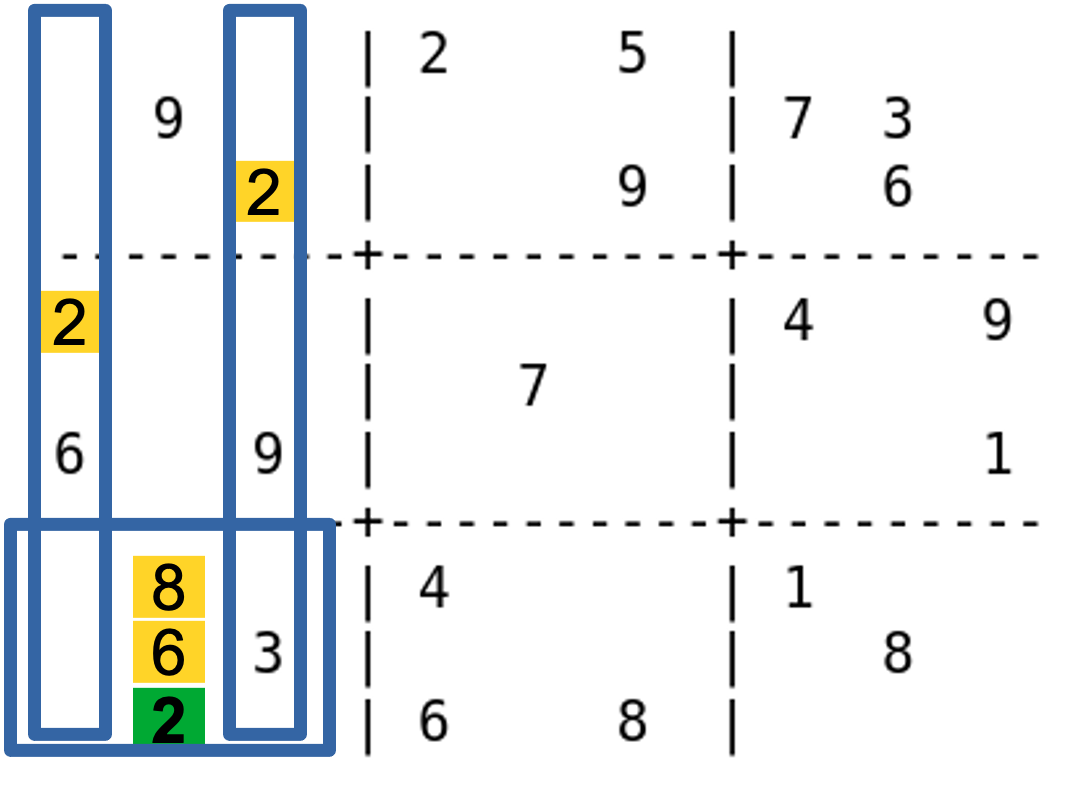
\includegraphics[width=0.8\textwidth]{figures/sudoku_steps/sudoku3}
				\end{figure}
			\end{minipage}
					\begin{minipage}{0.1\textwidth}
			\begin{center}
				$\rightarrow$
			\end{center}
		\end{minipage}
			\begin{minipage}{0.3\textwidth}
								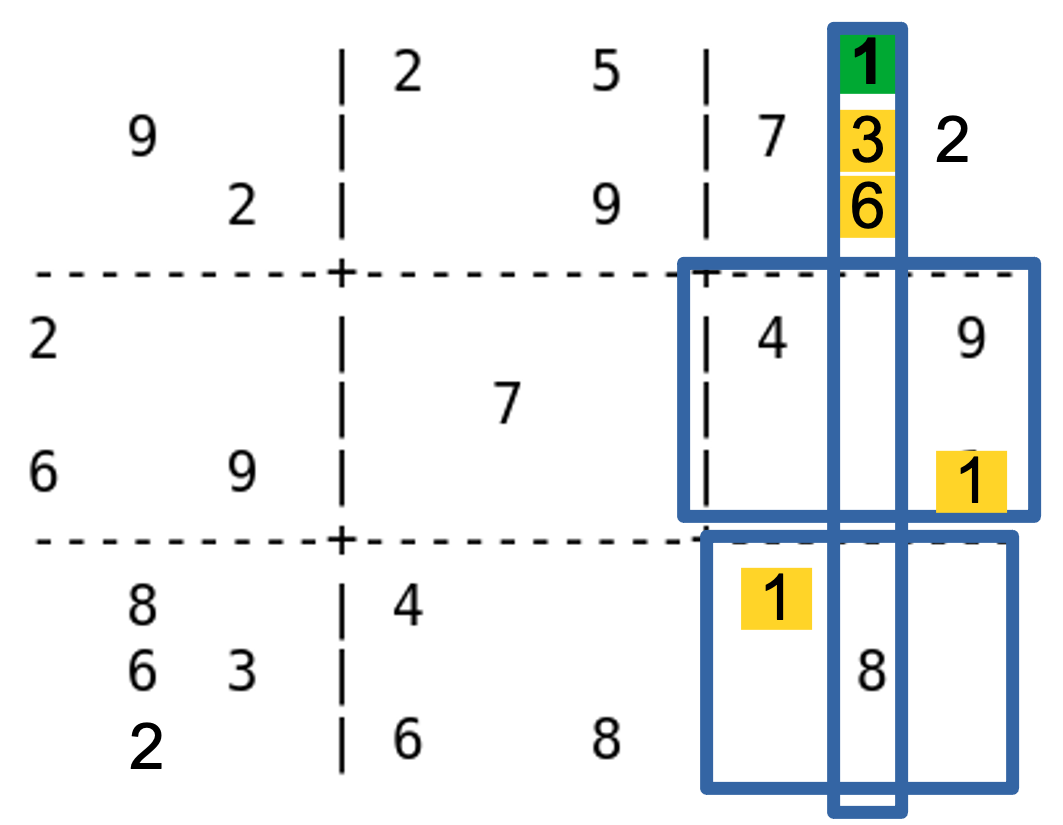
\includegraphics[width=0.8\textwidth]{figures/sudoku_sequence/sudoku-step3.png}
	\end{minipage}\hfill
				\begin{minipage}{0.095\textwidth}
\end{minipage}

\vfill		
		\begin{itemize}
			\item[{
\includegraphics[width=10pt]{figures/explanation_steps/explanation_S_full}}] Model constraints \pause
			%	\begin{itemize}
				\item \emph{Do not change} from an explanation step to another \pause
				%	\end{itemize}
			\item[{
\includegraphics[width=10pt]{figures/explanation_steps/explanation_E_full}}] Derived facts ${E}$  \pause
			%	\begin{itemize}
				\item \emph{Precision-increasing !}
				%	\end{itemize}
			
		\end{itemize}		
				\vfill		
			\end{frame}
			
			
			
			\begin{frame}{Incrementality}
				
%					\begin{algorithm}[H]
%						
%						\DontPrintSemicolon
%						\emph{\bf  $\setstohit  \gets \dots$} \tcp*{\emph{Collection of sets to hit}}
%						\While{\color{gray} true}{
%							$\subsetT \gets \cohs(\emph{\setstohit},f,p) $  \;
%							\color{gray}
%							\If{\color{gray} $\lnot \sat(\subsetT)$}{
%								\Return{\color{gray}$\subsetT$} \tcp*{OCUS found!}
%							}
%							{\color{black}$\setstohit  \gets \setstohit  \cup \emph{ \corrss( \subsetT, \formula)}$ } \;
%						}
%						\caption{$\comus(\formula,f,p)$ }
%						\label{alg:comus}
%					\end{algorithm}
%				\pause
%				\vfill
\textbf{Kick-start OCUS by bootstrapping $\m{H}$}
				\begin{itemize}
					\item[$\triangleright$] Keep track of collection of correction sets $\m{H}$ that need to be hit \pause
					\item[$\triangleright$] Each set H in \m{H} is the complement (with respect to the formula at hand) of a \emph{satisfiable subset} \pause
					\begin{itemize}
						\item[$\rightarrow$] Keep track of \emph{set of Satisfiable Subsets \textbf{SSs}} \pause
						\item[$\rightarrow$] Bootstrap $\m{H} \gets \{\m{F} \setminus \m{S} | \m{S}  \in  \mathbf{SSs} \}$ 
					\end{itemize}					
				\end{itemize}
				\textbf{In practice!}
				\begin{itemize}
					\item Incremental OCUS works with the full unsatisfiable formula of step 0
					\begin{itemize}
						\item $S \wedge E_{end} \wedge \{ \lnot n | n \in E_{end} \setminus E_{0}\}$
					\end{itemize}
					\item Initialize hitting set solver once and modify objective at every explanation step $i$ such that:
					\begin{itemize}
						\item Underived literal cannot be taken 
						\item Negated literals already explained cannot selected
					\end{itemize} 
				\end{itemize}
			\end{frame}
			
		\section{Results}
		 \begin{frame}
			\tableofcontents[currentsection]
		\end{frame}			
		\begin{frame}{Results - Explanation quality}

				\begin{minipage}{0.5\textwidth}
										\begin{center}
						{\Large $\mathtt{\mathbf{MUS}}$}\\ 
						$\downarrow$\\
						{\Large $\emph{\mathtt{\mathbf{OCUS}}}$}
					\end{center}	
				
%					\begin{center}
%						{\Large $\mathtt{\mathbf{MUS}}($}{\large 
\includegraphics[width=10pt]{figures/explanation_steps/explanation_S_full} $\&$ {
\includegraphics[width=10pt]{figures/explanation_steps/explanation_E_full}} $\& \lnot$ {
\includegraphics[width=10pt]{figures/explanation_steps/explanation_N}} $)$ } \\ 
%						$\downarrow$\\
%						{\Large $\emph{\mathtt{\mathbf{OCUS}}}($}{\large 
\includegraphics[width=10pt]{figures/explanation_steps/explanation_S_full} $\&$ {
\includegraphics[width=10pt]{figures/explanation_steps/explanation_E_full}} $\& \lnot$ {
\includegraphics[width=10pt]{figures/explanation_steps/explanation_N}} $, \emph{\mathbf{f}}, \emph{\mathbf{p}})$ } 
%					\end{center}				
				\end{minipage}
				\begin{minipage}{0.49\textwidth}
				\includegraphics[width=\textwidth]{figures/experiments/heatmapcosts_ocus_mus_2022070718.pdf}
					\end{minipage}

		\end{frame}
	
	
		
		\begin{frame}{Results - Correction Subset Enumeration}
%			\begin{minipage}{0.59\textwidth}
%				\begin{figure}[H]
%	\includegraphics[width=\textwidth]{figures/rq2_cactus_log_2022_06_27_OUS_IterLit_Incr_HS.pdf}
%\end{figure}
%
%			\end{minipage}
%			\begin{minipage}{0.4\textwidth}
%				\begin{figure}[H]
%	\includegraphics[width=0.9\textwidth]{figures/grow_types}
%\end{figure}
%\end{minipage}


									\begin{minipage}{0.45\textwidth}
	\begin{figure}
	\includegraphics[width=\textwidth]{figures/rq2_cactus_log_2022_06_27_OUS_IterLit_Incr_HS.pdf}
	\end{figure}
\end{minipage}\hfill
\begin{minipage}{0.53\textwidth}
	{\footnotesize
		\begin{algorithm}[H]		
			\DontPrintSemicolon
			\vspace{10pt}
			{\bf  $\setstohit  \gets \emptyset$} \;
			\While{\color{gray} true}{
				$\subsetT \gets \cohs({\setstohit},f,p) $  \;
				\color{gray}
				\If{\color{gray} $\lnot \sat(\subsetT)$}{
					\Return{\color{gray}$\subsetT$} \; 
				}
				{\color{black}$\setstohit  \gets \setstohit  \cup \emph{ \corrss( \subsetT, \formula)}$ } \;
			}
			\caption{$\comus(\formula,f,p)$ }
			\label{alg:comus}
		\end{algorithm}
	}
%\begin{figure}
%	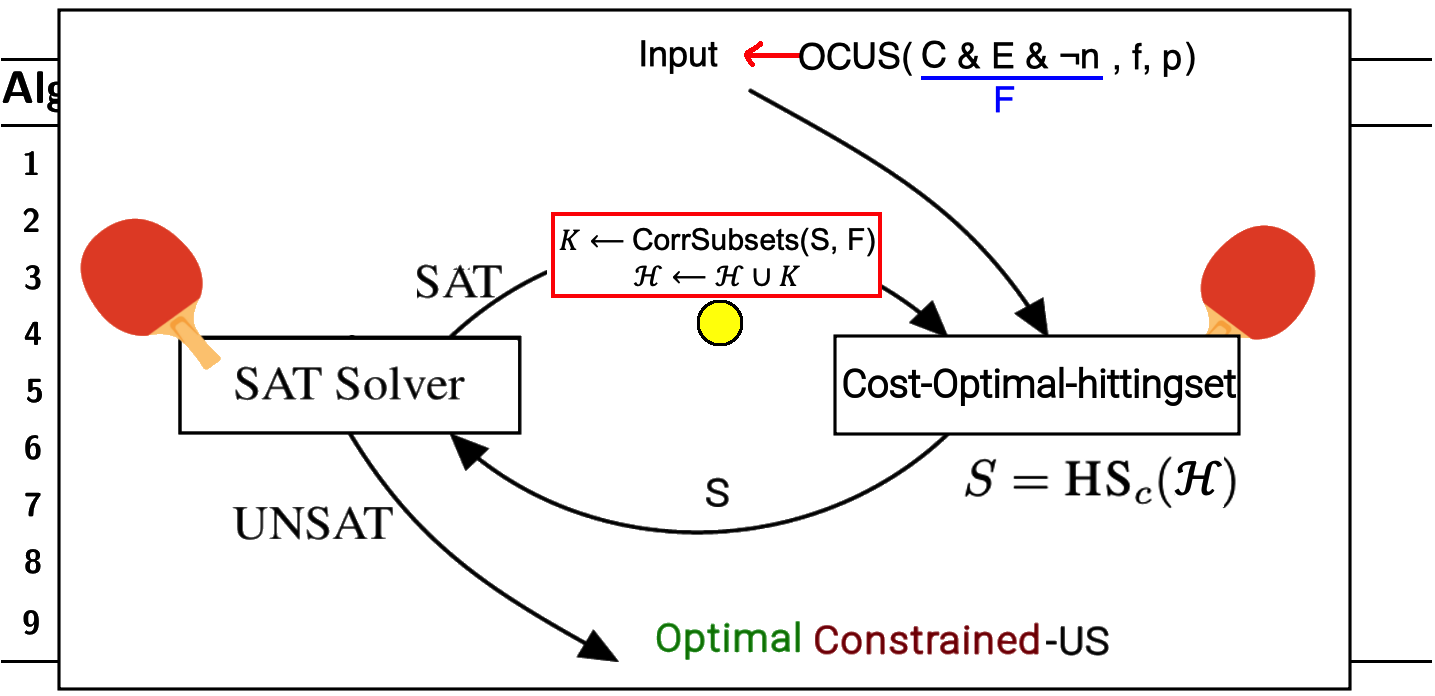
\includegraphics[width=0.8\textwidth]{figures/ping_pong/algo_with_ping_pong2b.png}
%\end{figure}
\end{minipage}

		\end{frame}
		
		
		\begin{frame}{Results - Incrementality}
			
									\begin{minipage}{0.42\textwidth}
				\begin{figure}
					\includegraphics[width=\textwidth]{figures/experiments/incremental_vs_non_SAT_2022_06_22.pdf}
				\end{figure}
			\end{minipage}\hfill
									\begin{minipage}{0.54\textwidth}
							{\footnotesize
								\begin{algorithm}[H]		
			\DontPrintSemicolon
			\emph{\bf  $\setstohit  \gets \dots$} \;
			\While{\color{gray} true}{
				$\subsetT \gets \cohs(\emph{\setstohit},f,p) $  \;
				\color{gray}
				\If{\color{gray} $\lnot \sat(\subsetT)$}{
					\Return{\color{gray}$\subsetT$} \; 
				}
				{\color{black}$\setstohit  \gets \setstohit  \cup { \corrss( \subsetT, \formula)}$ } \;
			}
			\caption{$\comus(\formula,f,p)$ }
			\label{alg:comus}
		\end{algorithm}
}
	\end{minipage}

		\end{frame}
			

		
		
		\section{Conclusion and Future work}
		 \begin{frame}
			\tableofcontents[currentsection]
		\end{frame}			
		
		\begin{frame}{Conclusion}
			We introduce \emph{\underline{O}ptimal \underline{C}onstrained} \underline{U}nsatisfiable \underline{S}ubsets (OCUS) problem and solved it using the \emph{implicit hitting set duality} between {\color{blue}MCSes} and {\color{teal}MUSes}.
			\vfill
			\begin{description}
				\item[Optimality] Cost-function quantifies explanation difficulty. \pause
				\item[Constrainedness] Impose structural constraints on the form of the explanations.\pause
				\item[Incrementality] Reuse-information between successive explanation calls.
				%		\item[Efficiency] 
				%		\begin{enumerate}
					%			\item Explanation-specific grow;
					%			\item Bound and sort OUS calls
					%		\end{enumerate}
			\end{description}
			\vfill
		\end{frame}
		
		
		\begin{frame}%{Use cases}
				\begin{center}\Large
					What can OCUS do for YOU ? 
				\end{center}
				\begin{figure}
					\centering
					
\includegraphics[width=0.2\textwidth]{figures/i_want_you_ocus.png}
				\end{figure}\pause
				\begin{itemize}
					\item Explaining scheduling, configuration problems .... and puzzles  \Cooley
					\item Debugging \textit{unsatisfiable models} with \emph{preferences} on the constraints \pause
					\item Stepwise explaining unsatisfiability \pause	
					\item Explaining Optimality for Constraint Optimization Problems 
					\begin{itemize}
						\item Why is the objective value not better ? 
					\end{itemize}

				\end{itemize}
			\end{frame}
				\begin{frame}{Future work}
			
			\begin{itemize}
				\item[$\triangleright$] What is a good cost-function to quantify how difficult an explanation is ? (from humans)
				\item[$\triangleright$] Explaining optimization (different types of ``why'' queries); close relation to Explainable AI Planning \cite{fox2017explainable}
				\item[$\triangleright$] Scaling up (approximate algorithms; decomposition of explanation search)
				%				\item[$\triangleright$] Incremental algorithms over different ``why'' queries
				% \item 
			\end{itemize}	
			
			
		\end{frame}
		
		\begin{frame}
			\frametitle{Future work}
			
			\begin{minipage}{0.28\textwidth}
				\includegraphics[width=\textwidth]{figures/sudoku_sequence/sudoku-step1}
			\end{minipage}\hfill
			\begin{minipage}{0.045\textwidth}
				\begin{center}
					$\rightarrow$
				\end{center}
			\end{minipage}\hfill
			\begin{minipage}{0.28\textwidth}
				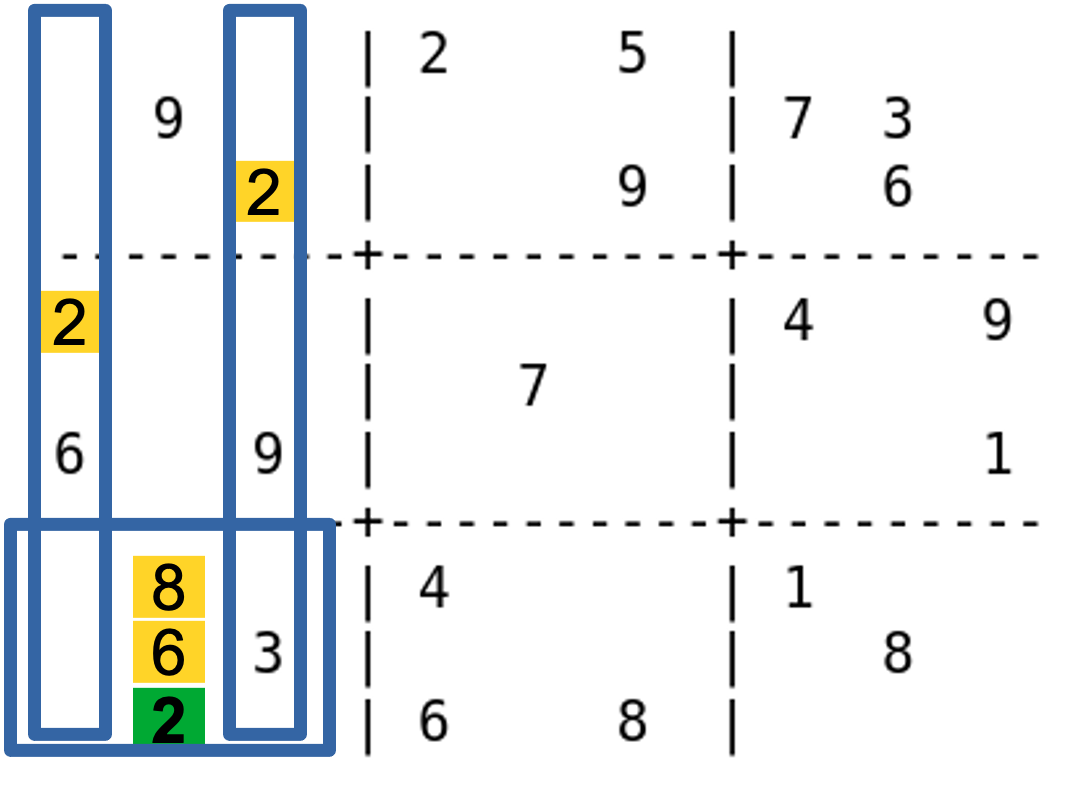
\includegraphics[width=\textwidth]{figures/sudoku_steps/sudoku3}
			\end{minipage}\hfill
			\begin{minipage}{0.045\textwidth}
				\begin{center}
					$\rightarrow$
				\end{center}
			\end{minipage}\hfill
			\begin{minipage}{0.28\textwidth}
				\begin{center}
					$\dots$
				\end{center}
			\end{minipage}\\\vfill 
			\begin{minipage}{0.28\textwidth}
				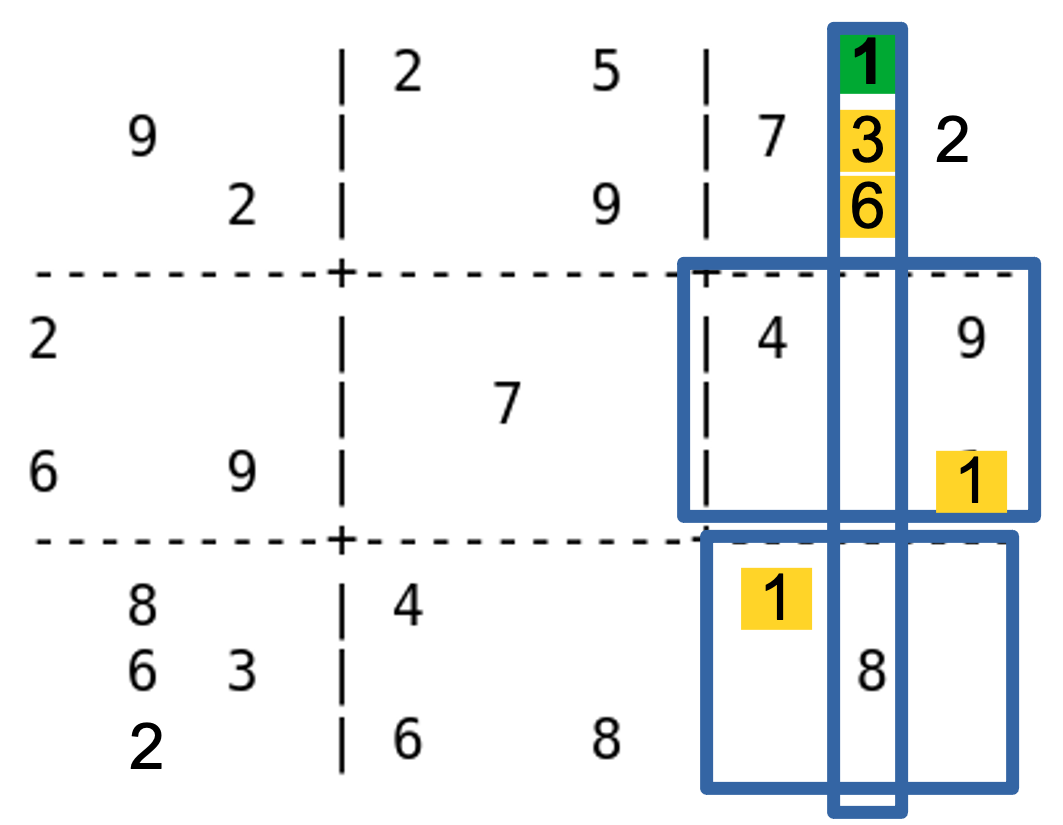
\includegraphics[width=\textwidth]{figures/sudoku_sequence/sudoku-step3}
			\end{minipage}
			\hfill
			\begin{minipage}{0.43\textwidth}
				\begin{center}
					$\rightarrow$ \hspace{0.5cm}\dots \hspace{0.5cm}$\rightarrow$
				\end{center}
			\end{minipage}\hfill
			\begin{minipage}{0.28\textwidth}
				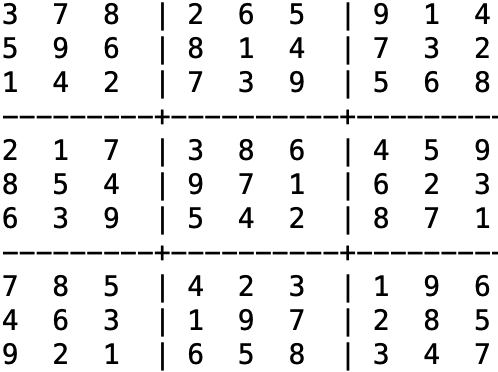
\includegraphics[width=\textwidth]{figures/sudoku_sequence/sudoku-stepn}
			\end{minipage}
		\end{frame}
		

		
		\begin{frame}{This is joint work with ... }
			
%		\vfill			
			\vspace{1.5cm}
\begin{minipage}{0.315\textwidth}
				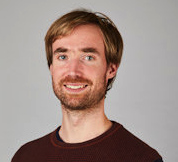
\includegraphics[width=\textwidth]{figures/tias.jpg}
		\end{minipage} \hfill
		\begin{minipage}{0.29\textwidth}
		
\includegraphics[width=\textwidth]{figures/frame}
	\end{minipage}\hfill
		\begin{minipage}{0.29\textwidth}
		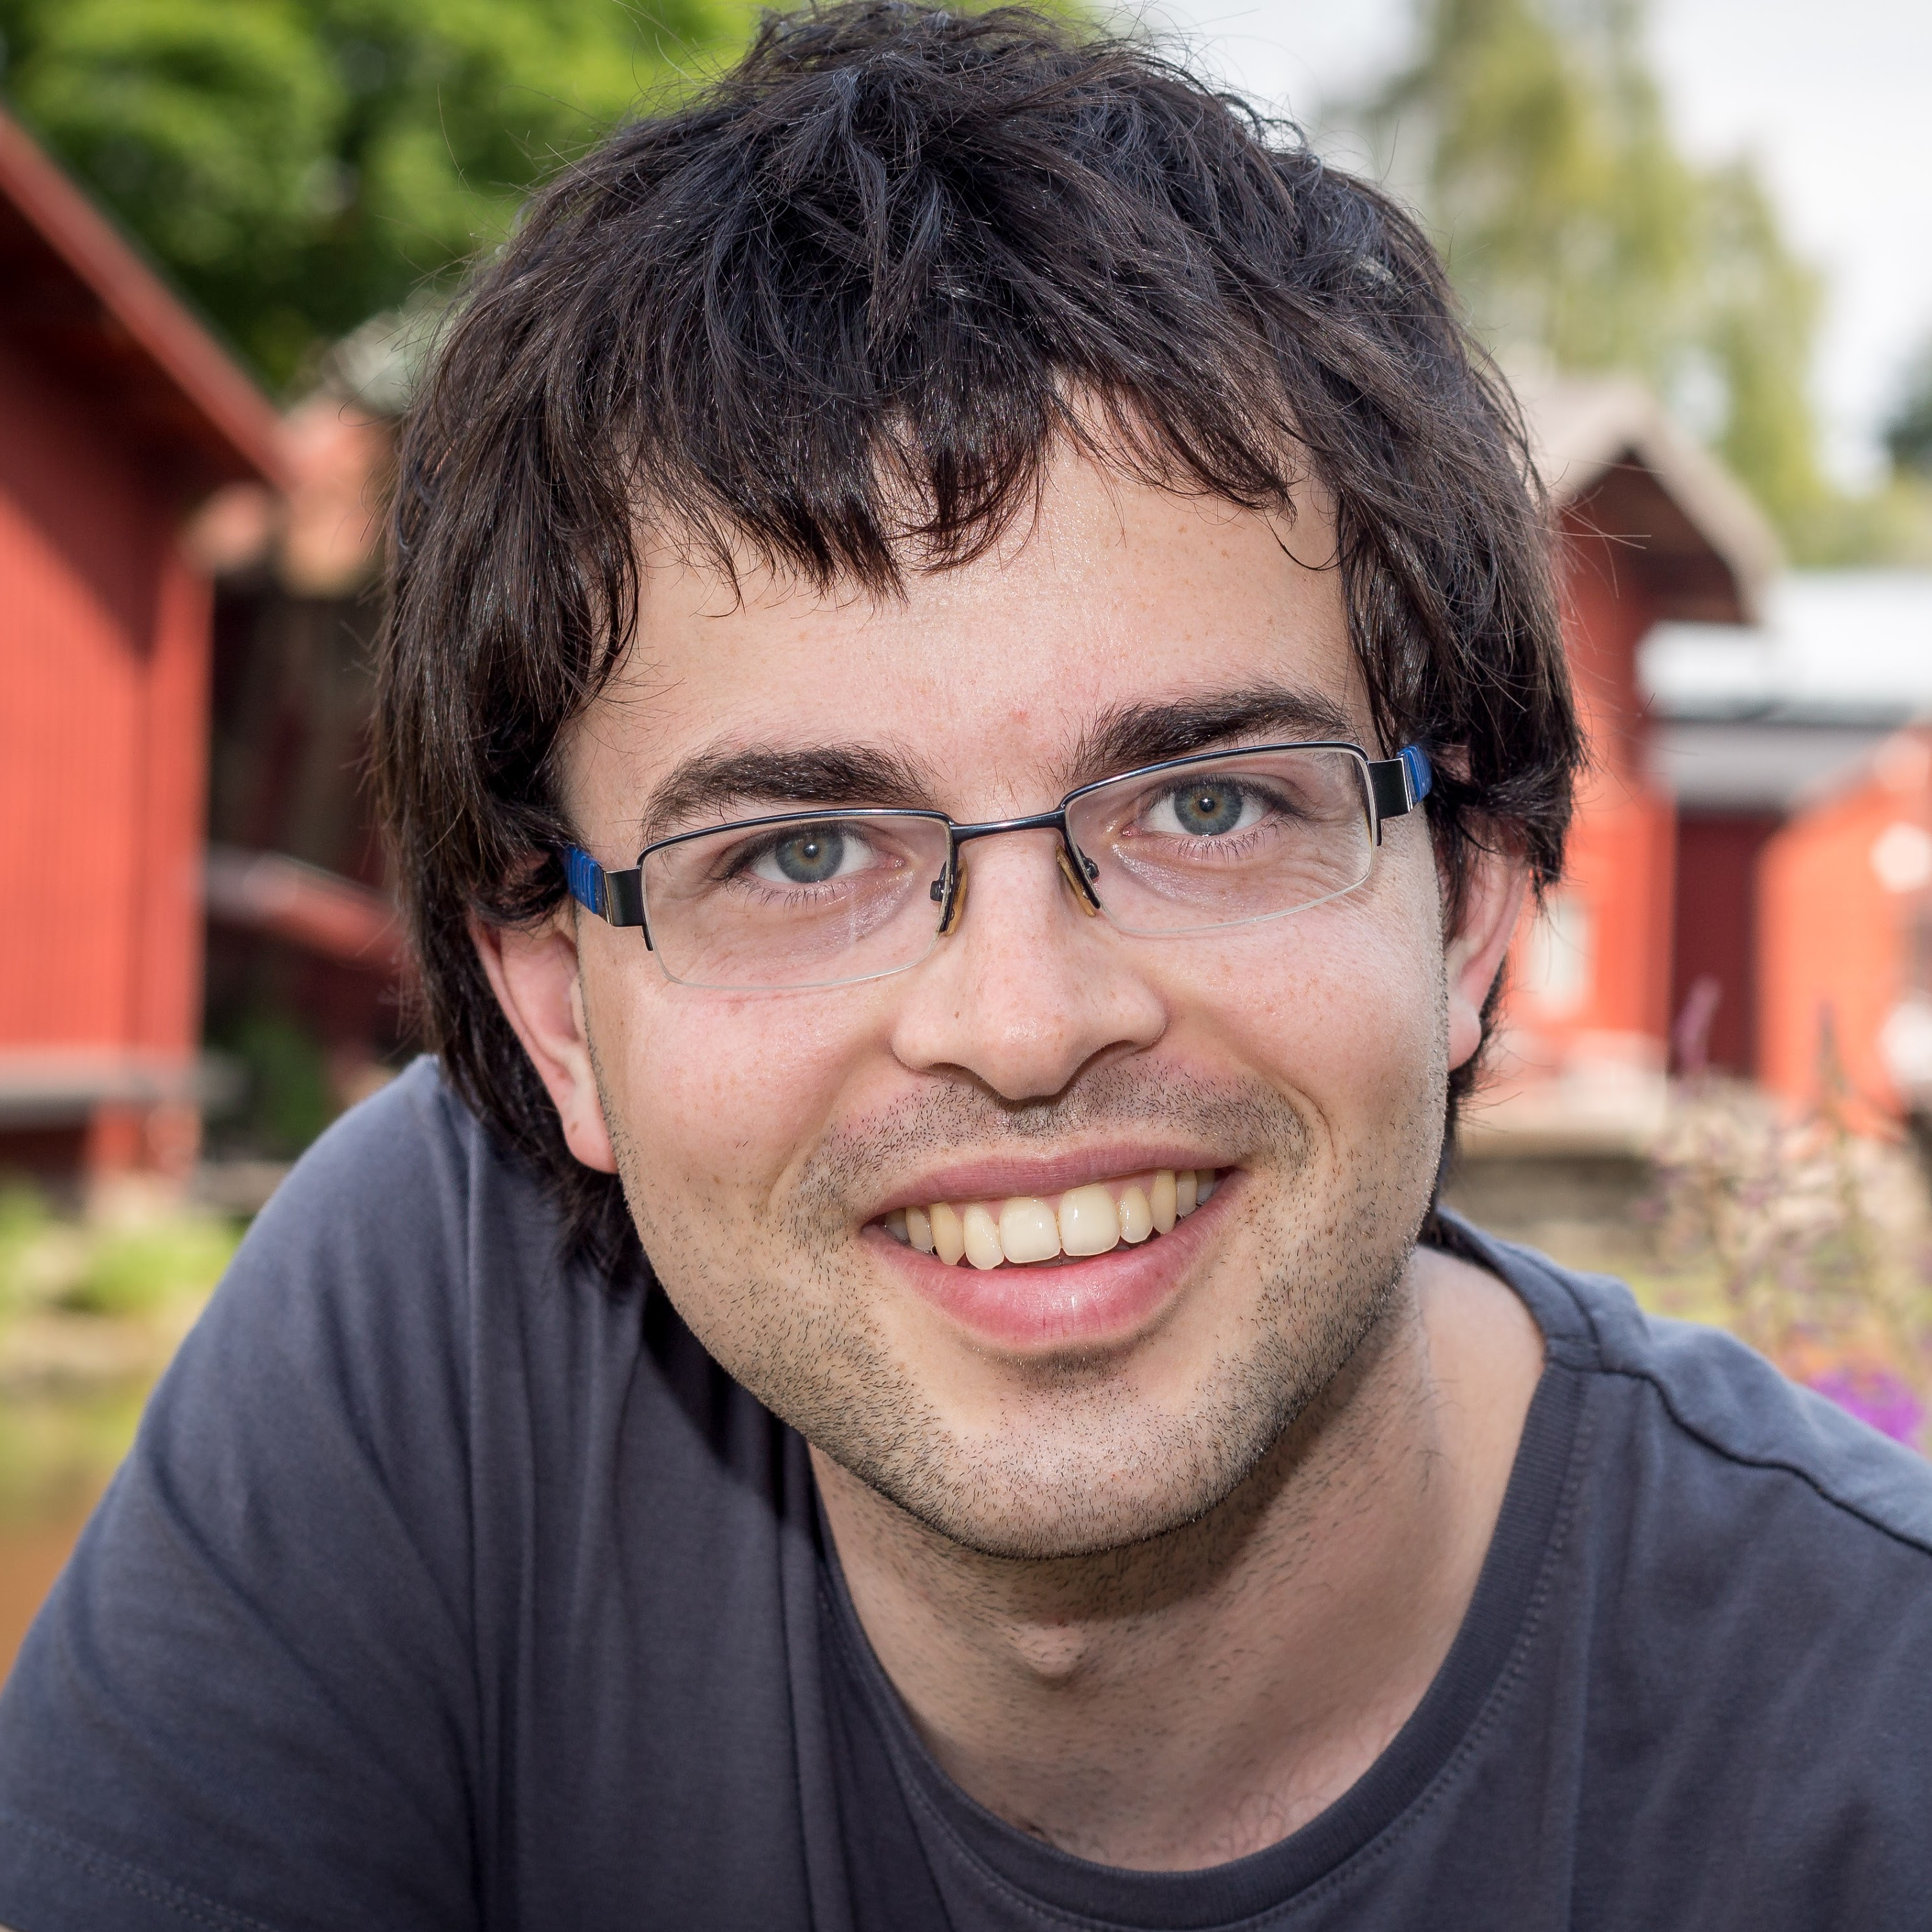
\includegraphics[width=\textwidth]{figures/bart.jpg}
	\end{minipage}	
	\begin{center}
		Emilio GAMBA \\
		\url{emilio.gamba@vub.be} 
%%		\\
%		\url{https://www.linkedin.com/in/emilio-g-9b1318140/}\\
	\end{center}
%		\vfill
		\vspace{0.5cm}
				\begin{minipage}{0.1\textwidth}
			
\includegraphics[width=\textwidth]{figures/datalab_400x400.jpg}
		\end{minipage}		\hfill
				\begin{minipage}{0.35\textwidth}
			\begin{flushleft}
				
\includegraphics[width=\textwidth]{template_vub/VUB-AI_RGB-1-800x223}
			\end{flushleft}
		\end{minipage}		\hfill
		\begin{minipage}{0.15\textwidth}
			
			
\includegraphics[width=\textwidth]{figures/DTAI_Logo_2}
		\end{minipage}

		\end{frame}
		
		
		\begin{frame}[allowframebreaks]
			\frametitle{References}
			\bibliographystyle{named}
			\bibliography{refs,references}
		\end{frame}
		
		
		
		
		
	\end{document}
	
	
	
	
	
	
	
	
	
